\documentclass[twoside]{article}

\usepackage{aistats2023}

% If your paper is accepted, change the options for the package
% aistats2023 as follows:
%
%\usepackage[accepted]{aistats2023}
%
% This option will print headings for the title of your paper and
% headings for the authors names, plus a copyright note at the end of
% the first column of the first page.

% If you set papersize explicitly, activate the following three lines:
%\special{papersize = 8.5in, 11in}
%\setlength{\pdfpageheight}{11in}
%\setlength{\pdfpagewidth}{8.5in}



% If you use BibTeX in apalike style, activate the following line:
% \bibliographystyle{apalike}
%% TODO make pdg.sty file that allows you to import all PDG macros.
%%%%%%%%%%


\relax % Writing Tools
    \newcommand{\TODO}[1][INCOMPLETE]{{\color{red}\hangindent=0.5cm\rightskip=0.8cm$\smash{\Big\langle}$~\texttt{#1}~\raisebox{-0.3ex}{${\Big\rangle}$}\hspace{-1.5cm}\par}}


\relax
	\DeclareMathOperator*{\argmin}{arg\,min}
	\newcommand{\bundle}{\mathbin{+}}
    \newcommand{\Rext}{\mskip1mu\overline{\mskip-1mu\mathbb R\!}\,}

\relax
    %% Narrowing
    \usepackage{keyval}
    \makeatletter
    \define@key{setpar}{left}[0pt]{\leftmargin=#1}
    \define@key{setpar}{right}[0pt]{\rightmargin=#1}
    \define@key{setpar}{both}{\leftmargin=#1\relax\rightmargin=#1}
    \makeatother

    \newenvironment{narrow}[1][]
      {\list{}{\setkeys{setpar}{left,right}%
         \setkeys{setpar}{#1}%
         \listparindent=\parindent
         \topsep=0pt
         \partopsep=0pt
         \parsep=\parskip}\item\relax\hspace*{\listparindent}\ignorespaces}
      {\endlist}
    % \newenvironment{abstract}
    %     {\narrow[both=1in]\small}         
    %     {\endnarrow}


\relax % Bibliography
    \usepackage[backend=biber, style=authoryear]{biblatex}
    % \usepackage[backend=biber,style=authoryear,hyperref=true]{biblatex}
    \addbibresource{refs.bib}

    \DeclareLanguageMapping{american}{american-apa}
    % \renewcommand*{\nameyeardelim}{\addcomma\space}
    \DeclareDelimFormat{nameyeardelim}{\addcomma\space}
    % \listfiles

    \DeclareFieldFormat{citehyperref}{%
      \DeclareFieldAlias{bibhyperref}{noformat}% Avoid nested links
      \bibhyperref{#1}}

    \DeclareFieldFormat{textcitehyperref}{%
      \DeclareFieldAlias{bibhyperref}{noformat}% Avoid nested links
      \bibhyperref{%
        #1%
        \ifbool{cbx:parens}
          {\bibcloseparen\global\boolfalse{cbx:parens}}
          {}}}

    \savebibmacro{cite}
    \savebibmacro{textcite}

    \renewbibmacro*{cite}{%
      \printtext[citehyperref]{%
        \restorebibmacro{cite}%
        \usebibmacro{cite}}}

    \renewbibmacro*{textcite}{%
      \ifboolexpr{
        ( not test {\iffieldundef{prenote}} and
          test {\ifnumequal{\value{citecount}}{1}} )
        or
        ( not test {\iffieldundef{postnote}} and
          test {\ifnumequal{\value{citecount}}{\value{citetotal}}} )
      }
        {\DeclareFieldAlias{textcitehyperref}{noformat}}
        {}%
      \printtext[textcitehyperref]{%
        \restorebibmacro{textcite}%
        \usebibmacro{textcite}}}


\usepackage{tikz}
	\usetikzlibrary{positioning,fit,calc, decorations, arrows, shapes, shapes.geometric}
	\usetikzlibrary{cd}

	%%%%%%%%%%%%
	\tikzset{AmpRep/.style={ampersand replacement=\&}}
	\tikzset{center base/.style={baseline={([yshift=-.8ex]current bounding box.center)}}}
	\tikzset{paperfig/.style={center base,scale=0.9, every node/.style={transform shape}}}

	% Node Stylings
	\tikzset{dpadded/.style={rounded corners=2, inner sep=0.7em, draw, outer sep=0.3em, fill={black!50}, fill opacity=0.08, text opacity=1}}
	\tikzset{dpad0/.style={outer sep=0.05em, inner sep=0.3em, draw=gray!75, rounded corners=4, fill=black!08, fill opacity=1, align=center}}
	\tikzset{dpadinline/.style={outer sep=0.05em, inner sep=2.5pt, rounded corners=2.5pt, draw=gray!75, fill=black!08, fill opacity=1, align=center, font=\small}}

 	\tikzset{dpad/.style args={#1}{every matrix/.append style={nodes={dpadded, #1}}}}
	\tikzset{light pad/.style={outer sep=0.2em, inner sep=0.5em, draw=gray!50}}

	\tikzset{arr/.style={draw, ->, thick, shorten <=3pt, shorten >=3pt}}
	\tikzset{arr0/.style={draw, ->, thick, shorten <=0pt, shorten >=0pt}}
	\tikzset{arr1/.style={draw, ->, thick, shorten <=1pt, shorten >=1pt}}
	\tikzset{arr2/.style={draw, ->, thick, shorten <=2pt, shorten >=2pt}}

	\newcommand\cmergearr[5][]{
		\draw[arr, #1, -] (#2) -- (#5) -- (#3);
		\draw[arr, #1, shorten <=0] (#5) -- (#4);
		}
	\newcommand\mergearr[4][]{
		\coordinate (center-#2#3#4) at (barycentric cs:#2=1,#3=1,#4=1.2);
		\cmergearr[#1]{#2}{#3}{#4}{center-#2#3#4}
		}
	\newcommand\cunmergearr[5][]{
		\draw[arr, #1, -, shorten >=0] (#2) -- (#5);
		\draw[arr, #1, shorten <=0] (#5) -- (#3);
		\draw[arr, #1, shorten <=0] (#5) -- (#4);
		}
	\newcommand\unmergearr[4][]{
		\coordinate (center-#2#3#4) at (barycentric cs:#2=1.2,#3=1,#4=1);
		\cunmergearr[#1]{#2}{#3}{#4}{center-#2#3#4}
		}


\relax %% Double delimeters; I need this for pdg macros \aar and \bbr
    \newcommand{\nhphantom}[2]{\sbox0{\kern-2%
    \nulldelimiterspace$\left.\delimsize#1\vphantom{#2}\right.$}\hspace{-.97\wd0}}
    % \nulldelimiterspace$\left.\delimsize#1%
    % \vrule depth\dp#2 height \ht#2 width0pt\right.$}\hspace{-.97\wd0}}
    \makeatletter
    \newsavebox{\abcmycontentbox}
    \newcommand\DeclareDoubleDelim[5]{
    \DeclarePairedDelimiterXPP{#1}[1]%
        {% box must be saved in this pre code
            \sbox{\abcmycontentbox}{\ensuremath{##1}}%
        }{#2}{#5}{}%
        %%% Correct spacing, but doesn't work with externalize.
        % {\nhphantom{#3}{##1}\hspace{1.2pt}\delimsize#3\mathopen{}##1\mathclose{}\delimsize#4\hspace{1.2pt}\nhphantom{#4}{##1}}
        %%% Fast, but wrong spacing.
        % {\nhphantom{#3}{~}\hspace{1.2pt}\delimsize#3\mathopen{}##1\mathclose{}\delimsize#4\hspace{1.2pt}\nhphantom{#4}{~}}
        %%% with savebox.
        {%
            \nhphantom{#3}{\usebox\abcmycontentbox}%
            \hspace{1.2pt} \delimsize#3%
            \mathopen{}\usebox{\abcmycontentbox}\mathclose{}%
            \delimsize#4\hspace{1.2pt}%
            \nhphantom{#4}{\usebox\abcmycontentbox}%
        }%
    }
    \makeatother

\relax %%%%%%%%%   PDG  MACROS   %%%%%%%%
	\newcommand{\ssub}[1]{_{\!_{#1}\!}}
	
	% \newcommand{\bp}[1][L]{\mat{p}_{\!_{#1}\!}}
	% \newcommand{\bP}[1][L]{\mat{P}_{\!_{#1}\!}}
    \newcommand{\pdgunit}{\mathrlap{\mathit 1} \mspace{2.3mu}\mathit 1}
	
	\newcommand{\X}{\mathcal X}
	\newcommand{\V}{\mathcal V}
	\newcommand{\N}{\mathcal N}
	\newcommand{\Ed}{\mathcal E}
	\newcommand{\Ar}{\mathcal A}
	\newcommand{\ArST}{\hat\Ar}
	
    \newcommand{\balpha}{\boldsymbol\alpha}
    \newcommand{\bbeta}{\boldsymbol\beta}

	\newcommand{\bp}[1][L]{\mat{p}\ssub{#1}}
	\newcommand{\bP}[1][L]{\mat{P}\ssub{#1}}
	% \def\p_#1{p\ssub{#1}}
	\def\p_#1{\mathbb P_{#1}}	

	%%%%% a clever version of \Src,\Tgt, and \p that supresses subscripts
	\newif\ifsuba \subatrue
	\let\psimp\p  % \let\simpSrc\Src   \let\simpTgt\Tgt 
	% \renewcommand\Src[1]{\simpSrc{\ifsuba #1\fi}}
	% \renewcommand\Tgt[1]{\simpTgt{\ifsuba #1\fi}}
	\newcommand\Src[1]{\ifsuba S\mskip-2mu\vphantom{|}_{{#1}} \else S \fi}
	\newcommand\Tgt[1]{\ifsuba T\mskip-3mu\vphantom{|}_{{#1}} \else T \fi}
	% \def\p_#1(#2){\subafalse\psimp_{#1}(#2)\subatrue}

	% \newcommand\Src[1]{S\mskip-2mu\vphantom{|}_{{#1}}}
    % \newcommand\Tgt[1]{T\mskip-3mu\vphantom{|}_{{#1}}}	
    % \newcommand\Src[1]{X_{{#1}}}
    % \newcommand\Tgt[1]{Y_{{#1}}}
    % \newcommand{\Src}{\mathrm{Src}}
    % \newcommand{\Tgt}{\mathrm{Tgt}}
    % \newcommand\Src[1]{S\mskip-2mu\mathit{r\mskip-3muc}_{{#1}}}
    % \newcommand\Tgt[1]{T\mskip-5mu\mathit{g\mskip-1mut}_{{#1}}}
    % \newcommand\Src[1]{\mathsf{S}\mskip-2mu\vphantom{|}_{{#1}}}
    % \newcommand\Tgt[1]{\mathsf{T}\mskip-3mu\vphantom{|}_{{#1}}}
    

	\DeclareMathAlphabet{\mathdcal}{U}{dutchcal}{m}{n}
	\DeclareMathAlphabet{\mathbdcal}{U}{dutchcal}{b}{n}
	\newcommand{\dg}[1]{\mathbdcal{#1}}
	\newcommand{\PDGof}[1]{{\dg M}_{#1}}
	\newcommand{\UPDGof}[1]{{\dg N}_{#1}}
	\newcommand\VFE{\mathit{V\mkern-4mu F\mkern-4.5mu E}}

	\newcommand\Inc{\mathit{Inc}}
	\newcommand{\IDef}[1]{\mathit{IDef}_{\!#1}}
	\newcommand\OInc{\mathit{O\mskip-2.5muI\mskip-3.5mun\mskip-1.7muc}} % new version of Inc
	% \newcommand\CInc{\mathit{C\mskip-3.1muI\mskip-3.5mun\mskip-1.7muc}} % new version of IDef
	\newcommand\CDef{\mathit{C\mskip-3.5muD\mskip-2.5mue\mskip-1.5muf}} % new version of IDef
	% \newcommand{\SInc}{\mathit{S\mskip-1muI\mskip-1mun\mskip-1muc}} % new version of IDef
	% \newcommand{\ed}[3]{%
	% 	\mathchoice%
	% 	{#2\overset{\smash{\mskip-5mu\raisebox{-3pt}{${#1}$}}}{\xrightarrow{\hphantom{\scriptstyle {#1}}}} #3} %display style
	% 	{#2\overset{\smash{\mskip-5mu\raisebox{-3pt}{$\scriptstyle {#1}$}}}{\xrightarrow{\hphantom{\scriptstyle {#1}}}} #3}% text style
	% 	{#2\overset{\smash{\mskip-5mu\raisebox{-3pt}{$\scriptscriptstyle {#1}$}}}{\xrightarrow{\hphantom{\scriptscriptstyle {#1}}}} #3} %script style
	% 	{#2\overset{\smash{\mskip-5mu\raisebox{-3pt}{$\scriptscriptstyle {#1}$}}}{\xrightarrow{\hphantom{\scriptscriptstyle {#1}}}} #3}} %scriptscriptstyle
	\newcommand{\ed}[3]{#2%
	  \overset{\smash{\mskip-5mu\raisebox{-1pt}{$\scriptscriptstyle
	        #1$}}}{\rightarrow} #3}

	\newcommand{\bundle}{\mathbin{+}}
	\DeclareDoubleDelim
		\SD\{\{\}\}
	\DeclareDoubleDelim
		\bbr[[]]
	% \DeclareDoubleDelim
	% 	\aar\langle\langle\rangle\rangle
	\makeatletter
	\newsavebox{\aar@content}
	\newcommand\aar{\@ifstar\aar@one@star\aar@plain}
	\newcommand\aar@one@star{\@ifstar\aar@resize{\aar@plain*}}
	\newcommand\aar@resize[1]{\sbox{\aar@content}{#1}\scaleleftright[3.8ex]
		{\Biggl\langle\!\!\!\!\Biggl\langle}{\usebox{\aar@content}}
		{\Biggr\rangle\!\!\!\!\Biggr\rangle}}
	\DeclareDoubleDelim
		\aar@plain\langle\langle\rangle\rangle
	\makeatother


	% \DeclarePairedDelimiterX{\aar}[1]{\langle}{\rangle}
	% 	{\nhphantom{\langle}{#1}\hspace{1.2pt}\delimsize\langle\mathopen{}#1\mathclose{}\delimsize\rangle\hspace{1.2pt}\nhphantom{\rangle}{#1}}


\colorlet{mayyybe}{blue!50!red!20!white}

% \author{$\{$Oliver E Richardson, Joseph Y Halpern, Christopher De Sa$\}$}

\begin{document}
% If your paper is accepted and the title of your paper is very long,
% the style will print as headings an error message. Use the following
% command to supply a shorter title of your paper so that it can be
% used as headings.
%
%\runningtitle{I use this title instead because the last one was very long}

% If your paper is accepted and the number of authors is large, the
% style will print as headings an error message. Use the following
% command to supply a shorter version of the authors names so that
% they can be used as headings (for example, use only the surnames)
%
%\runningauthor{Surname 1, Surname 2, Surname 3, ...., Surname n}

\twocolumn[

%joe1: I would cut the second part of the title
%  \aistatstitle{Inference in Probabilistic Dependency Graphs,\\
  %    via Exponential Cones and Otherwise}
  %oli3:
    % \aistatstitle{Inference in Probabilistic Dependency Graphs}
    \aistatstitle{Inference in Probabilistic Dependency Graphs,\\
        via Exponential Conic Programming
        }

%joe1: initials need periods
    %\aistatsauthor{ Oliver E Richardson \And Joseph Y Halpern \And
    \aistatsauthor{ Oliver E. Richardson \And Joseph Y. Halpern \And
  Christopher De Sa }
% \aistatsaddress{ Institution 1 \And  Institution 2 \And Institution 3 }
\aistatsaddress{Cornell University \And Cornell University \And Cornell University}
]

\begin{abstract}
    We provide the first tractable inference algorithm for
    Probabilistic Dependency Graphs (PDGs) with discrete variables,
    thereby placing PDGs on asymptotically similar footing as other
%joe1
%    graphical models, such as Bayesian Networks and Factor Graphs.
    %    This may be surprising, because PDGs are more expressive than
graphical models, such as Bayesian Networks and Factor Graphs,
%oli3
% despite the fact that PDGs are significantly more expressive
% than other probabilistic graphical models.
despite the fact that PDGs are more expressive.
%joe1: I have no idea what you mean by "a PDG inferencd algorithm can
%be used to calibrate a broad class of statistical models."  Since I
%don't think you discuss this issue anywhere in the paper, I just cut it.
%other probabilistic graphical models, and also because a PDG
%    inference algorithm can be used
%    % for ``inconsistency minimization'',
%    % which has been argued to be widely useful.
%    % to resolve inconsistencies, which has  as a generic modeling task.
%    % as a black box to train statistical models in ML.
%    to calibrate a broad class of statistical models.
%joe1: cut paragraph break
The key to our approach is combining
%joe
%(1) our finding that inference in PDGs with bounded tree-width can
(1) the observation that inference in PDGs with bounded tree-width can
be reduced to a tractable linear optimization problem with exponential
cone constraints,
%joe1
%with (2) a recent interior point method that can (provably) solve
with (2) a recent interior-point method that can solve
such problems efficiently (Dahl \& Anderson, 2022).
%joe1: say something about how you do the evaluation; just showing how
%it does on random PDGs is nbot enough.  I don't think comparing it
%only to belief propagation is enough either.
%    We provide a concrete implementation and empirical evaluation.
We evaluate our approach by ...
%joe1: I wouldn't worry about hte other approaches now.  There are
%more important issues hou have to deal with first.
%    In addition, we prove auxiliary results about complexity of this
%    problem, and discuss other approaches to it.
% We also characterize the complexity of various components of the
% inference problem.
\end{abstract}


% \begin{narrow}
% %%-----------    A FRANK SUMMARY    ---------------
% Measuring / Estimating /  Inconsistency is very useful.
% For instance, (1) propagating it backwards through layers of computation = differentiable learning.
%
% Certain localized versions of it can be used to do other algorithms.

% How hard is it?
% With interior point methods (convex programs with exponential cone constraints) we can do it in $O(n^4 \log n)$ time \& space, worst case for exact inference. So far, this means slightly harder than inference in Graphical models.
% \end{narrow}


% \tableofcontents

\section{INTRODUCTION}


% {\color{gray}
% Suppose that we have a collection of probabilistic beliefs.
% How can we tell if they are self-consistent?
% How difficult is it to measure how inconsistent they are?
% How much computation is necessary to synthesize our beliefs into a single joint probability distribution?
% This paper provides answers---both
% theoretical and practical---to these questions. }
%joe3*: While these are interesting questions, they are not the
%standard questions tyhat have been asked when it comes to inference.
%since no other approach can capture inconsistency well, no one has
%asked the question of how inconsistent beliefs are (to the best of my
%knowledge). Moreover, the notion of inconsistency you're dealing
%with is an idiosyncratic notion, that you tailored to PDGs.   That
%means the leadoff paragraph does not situate this work well in the
%ocntext of what's been done.  It may be better to start with
%inference (what you denote as (Q)) and then move to inconsistency,
%rather than the other way around, as you've done.  I think that would
%make the story read better.
% {\color{mayyybe}
% hi
% }

% More concretely, we handle
Probabilistic Dependency Graphs, or PDGs \parencite{pdg-aaai},
are a particularly flexible class of probabilistic graphical models, which subsumes Bayesian Networks (BNs)
% and Markov Random Fields (MRFs).
and Factor Graphs (FGs).
%joe1: much too wordy
%The primary force behind the expressiveness of pdgs is their ability
%to capture inconsistent beliefs, and the natural way of measuring the
%degree of this inconsistency that the formalism provides.
Unlike the models they generalize,
PDGs can capture inconsistent beliefs, and have an associated measure
%oli2: I cut "of degree" and added quotes
% of degree of inconsistency that captures how far a PDG is from being consistent.
%oli3: making this less tautological
% of ``inconsistency'' that quantifies how far a PDG is from being consistent.
of ``inconsistency'' that quantifies how far the the probabilities in a PDG are from being self-consistent.
% Beyond its role in undergirding the semantics of pdgs,
% Beyond its role in providing the semantics of pdgs,
% Beyond its central role in the development of PDG semantics, this inconsistency measurement also captures many standard loss functions and statistical divergences \parencite{one-true-loss}.
But, also unlike the models they generalize,
PDGs have not had an inference algorithm---%
% there have been no practical algorithms that can answer
% probabilistic queries about the distribution a PDG represents.
there has been no practical way to use a PDG to compute answers to
probabilistic queries.
% respond to probabilistic queries.
This paper presents the first such algorithm.

Beyond its central role in the development of PDG semantics, this measure of inconsistency has proved broadly to be a natural quantity to minimize.
As shown by \textcite{one-true-loss},
 % a wide breadth of
many
    loss functions and statistical divergences
    % used in practice
    % arise as the inconsistency measurement
    can be viewed as measuring the inconsistency
    of a PDG that models the appropriate context.
So, the ability to calculate and minimize inconsistency seems eminantly useful.
It follows, for instance, that the training process in machine learning can largely be conceptualized as inconsistency minimization.
But how {does} one calculate this degree of inconsistency, in general?
% (let alone minimize it)?
Earlier work does not say.
%
This problem turns out to be closely related to inference in PDGs,
and our approach addresses both.
% These two practical shortcomings
% which have made PDGs a purely theoretical construct
% are related, and we provide an algorithm
% that addresses both.

Since inference in other graphical models is alredy NP-hard, the same must be true of the more general class of PDGs.
% The only hope for tractability is the same class of models
At a high level, the best we could hope for would be tractability on the restricted
class of models on which inference has traditionally been tractable---that is, a polynomial algorithm for models whose underlying structure has bounded tree-width.
That is precisely what we have.
% same class of graphical models
% a polynomial-time algorithm in the case of bounded tree-width.
% This is precisely what we prsent here.
% which means PDGs have the same type of fixed-parameter tractability enjoyed by
% BNs and FGs.
Interestingly, the constriction is not trivial.
% It is not a variant of belief propagation (BP), nor is it
%
% Unlike the many variants of exact inference
While the many approaches to exact inference in standard graphical models have largely turned out to be various perspectives on the same mathematics \parencite[\S9-11]{koller2009probabilistic},
% our approach has roots in a very different.
% our approach is quite different in nature.
our approach seems by all acounts to be quite different.
% and .
% new iterior point methods.

Our ability to do PDG inference in polynomial time is based on a line of recent work in convex programming that establishes polynomial-time convergence
\parencite{badenbroek2021algorithm,dahl2022primal}
for a class of problems called \emph{exponential conic programs}
\parencite{lubin}.
Our contribution here is to show that the problem of inference in a PDG can be efficiently converted to an exponential conic program, at which point it can be solved with a commercial solver \parencite{mosek} in polynomial time.
% We show that the problem of inference in a PDG can be efficiently converted to an exponential conic program, at which point it can be solved with a commercial solver \parencite{mosek} in polynomial time.
The direct appeal to a commercial solver gives us efficiency out of the box, and also allows us to benefit from future improvements in exponential conic optimization.
Thus our result is not only a theoretical one, but practical as well.


\textbf{Contributions.}
We provide the first algorithm to provably do inference in PDGs.
Better still, it is fixed-parameter tractable: for models of bounded treewidth,
    it runs in polynomial time.
We show how PDG inference can be reduced to conic exponential programming,
    in a way that can be offloaded to a powerful existing solvers.
We also provide a python implementation of the conversion in a standard convex optimization framework, thereby completing the software interface between such solvers and the standard library describing PDGs.
Finally, we evaluate this implementation empirically, and show that it is both more accurate and faster than other optimization baselines.
%
% Moreover, the approach makes use of , giving us efficiency out-of-the box.

\section{PRELIMINARIES AND RELATED WORK}

\textbf{Notation.}
% This paper concerns the
% Unless otherwise specified, all scalar quantites range over the extended reals $\Rext := \mathbb R \cup \{\infty\}$.
% For us, a vector is a map from a finite set to the extended reals
%     $\Rext := \mathbb R \cup \{\infty\}$.
For us, a vector is a map from a finite set to the extended reals
    $\Rext := \mathbb R \cup \{\infty\}$.
The \emph{shape} of a vector $\mat u$ is the finite set which is its domain.
% The notation $\mat u := [u_i]_{i \in S}$ defines a vector over the finite set $S$.
The notation $\mat u := [u_i]_{i \in S}$ defines a vector of shape $S$.
We will sometimes use superscripts as well, especially when indices depend on one another. For example, if $\dg S$ is a finite set of finite sets, then
%joe2: (1) why is this a disjoint union?  You never said that the sets in
%\X were disjoint.  (2) You don't want to include X \in \X and x
%\n X in the notation; it's really ugly.  I would slightly prefer
%u_{x,X}$.  (3) Technically, if it's a vector, you have to specify the
%order of the elements, and the notation doesn't do that.
%oli2: (1) This is one construction of the disjoint union. It doesn't matter if the sets
% X \in \X are disjoint; even if x is a member of X1 and X2, the indices (X1, x) and (X2,x) will be different.  (2) I agree that it's a little bit ugly, but I think leaving it out is far more confusing.  (3) Not necessarily.  Just because the standard basis (e_1, ... e_n) has an order doesn't mean we have to provide an order if we use a different basis. Sure, we need an order to write down a concrete vector without reference to the basis elements, but we won't need to do that.
% $\mat u := [u^X_x]^{X \in \mathcal X}_{x \in X}$ defines a vector whose indicies range over the disjiont union $\sqcup \mathcal X$.
%oli2: here's a compromise
% $[u^X_x]_{x \in X, X \in \X}$ denotes a vector which has an element
% for each $X \in \X$ and $x \in X$.
$[u^S_s]^{S \in \dg S}_{s \in S}$ denotes a vector which has an element
%oli2: futher clarifying now that you've stripped the "disjoint union" out...
% for each $X \in \mathcal X$ and $x \in X$.
for each pair $(S,s)$, satisfying $s \in S \in \dg S$.
 % for each $(X, x)$
%joe2: now you're really getting into the weeds.  This is a paper
%about inference, not notation.
%oli2: ok, although I think it's clearer to spell it out.
%It is equivalent to $\mat u := [u_{(x,X)}]_{x \in X, X \in \mathcal X}$, but more compact.
%joe2: I don't know what "the subspace where the upper index is $X$"
%means.  If you really need this notation, you need to explain it
%better.  But this is really the wrong place for it.
%oli2: if you can point out a better place for it later, that's ok.
% But I think this notation will be a distraction once we get into the actual
% story we want to tell.
% Supplying just the upper index, $\mat u^{X}$ is the projection of $\mat u$ onto the subspace where the upper index is $X$.
% Supplying just the upper index, $\mat u^{X_0} := [u^{X_0}_x]_{x \in {X_0}}$
% is the projection of $\mat u$ onto the subspace whose upper index is $X_0$.
By supplying just the upper index of such a vector, as in $\mat u^{S_0}$,
we mean $[u^{S_0}_s]_{s \in {S_0}}$, the projection of $\mat u$ onto the subspace whose upper index is $S_0$.
% Vectors over the same set
Vectors of the same shape
 can be added (+) and partially ordered ($\le$) pointwise as usual; pointwise multiplication is denoted by $\odot$.
$\mat 1$ denotes an all-ones vector, whose dimension will always be clear in context.
$\mat u^{\sf T}$ denotes the transpose of $\mat u$, which we use primarily to denote the inner product $\mat u^{\sf T} \mat v$.
% If $\mat u : A \to \Rext$ is a vetor over $A$, and $\mat v : A \times B \to \Rext$,
% then $\mat u \otimes \mat 1 : A \times \Gamma \to \Rext$, by
% $(\mat u \otimes \mat 1)(a,\gamma) := \mat u(\gamma)$
If $\mat u = [u_a]_{a \in A}$ is a vector over $A$ and $\mat v = [v_b]_{b \in B}$ is a vector over $B$, then $\mat u \mathbin{\otimes} \mat v := [ u_a \cdot v_b ]_{a \in A, b \in B}$ is a vector over $A \times B$.

% {\color{red}\tt
% TODO: unexplained notation / concepts
% \begin{enumerate}[nosep]
% \raggedright
% \item tensor product $\otimes$  (TODO: nix it)
% \item relative entropy $\kldiv\mu\nu$, conditional entropy $\H(Y|X)$
% \end{enumerate}
% }

\textit{Probabilities.}
We write $\Delta S$ to denote the set of probability distributions over a finite set $S$.
Every variable $X$ can take on values from a finite set $\V\mskip-1mu X$ of possible values.
% If $S$ is a finite set, we write $\Delta S$ for the set of probability distributions over $S$, i.e., the simplex over its elements.
A conditional probability distribution (cpd) $p(Y|X)$ is a map
%joe2
%$p : \V(X) \to \Delta \V(Y)$, so it assigns, to every $x \in \V(X)$, a
$p : \V\mskip-1mu  X \to \Delta \V Y$, so it assigns to each $x \in \V\mskip-1mu X$ a
probability distribution $p(Y|x) \in \Delta \V Y$, which is shorthand for $p(Y|X\!\!=\!x)$.
Given a joint distribution $\mu$ over many variables including both $X$ and $Y$,
%joe1: Is this standard notation for a marginal?  \mu)(X) looks like
%the probability of X to me.
%oli1: I'm pretty sure it's standard; at the very least, it agrees with the standard notation:  If you had Pr(X,Y), and you wanted to talk about the probability of X, you would write Pr(X), which is also the marginal of the distribution \Pr.
we write $\mu(X)$ for its marginal distribution on $X$,
% $\mu(X,Y)$ for the
and $\mu(Y|X)$ for the cpd obtained by first conditioning on $X$ and then marginalizing to $Y$.
We measure information in a distribution with entropy $\H(\mu) := \Ex_{\mu} [\log \frac1\mu]$ and conditional entropy $\H_\mu(Y|X) := \Ex_\mu[\log\nicefrac1{\mu(Y|X)}]$, where $X$ and $Y$ are variables.
% \textbf{Graph Theory.}

% \textbf{Inference for Graphical Models.}
% % A graphical model is a graph whose vertices correspond to
% %
% % There is a natural equivalence between hyper-graphs and bipartite graphs
% % \[
% % \]


% \textbf{Hypergraphs, Tree Decompositions, and Treewidth.}
\textbf{Hypergraphs and Treewidth.}
%joe2: what's the INTUITION for a hyperedge?
%oli2: I don't get why this is necessary. At this point it's just an analogue of a
% graph. Would you want me to give intuition for what an edge of a graph means in
% general, if it were slightly less standard?  It's useful generally.
A hypergraph $G = (V, \Ed)$ is a set $V$ of vertices, and a collection $\Ed$ of \emph{hyperedges}, which correspond to subsets of $V$.
% An ordinary graph may be regarded as the special case in which every hyperedge contains two vertices.
An ordinary graph may be viewed as the special case in which every hyperedge contains  two vertices.
% An ordinary graph may be viewed as the special case of a hypergraph in which every hyperedge contains exactly two vertices.
% There is a natural bijection between hyper-graphs and bipartite graphs.

\begin{defn}
    A \emph{directed hypergraph} $G = (N, \mathcal A)$ is a set $N$ of nodes, and a collection $\mathcal A$ of \emph{hyperarcs}; each $a \in \mathcal A$
    is associated with a set $\Src a \subset N$ of source nodes, and a set $\Tgt a \subset N$ target nodes.
\end{defn}
% A directed graph is just a directed hypergraph where the source and target sets of every hyperarc are singletons.
A directed graph can be seen a directed hypergraph in which every source and target set is a singleton.
%joe2
%As one might hope, we can form hypergraph from a directed hypergraph
% We can form a hypergraph from a directed hypergraph
In turn, a directed hypergraph can be seen as a hypergraph
by taking the union of the source and target sets,
thereby ``forgetting the direction of the arrow''.
% There is also a natural bijection between directed hypergraphs and directed bipartite graphs.

% Given a hyper-graph $(\X, \Ed)$,
Many problems that are intractable for general graphs
are tractable when restricted to trees.
some graphs are closer to trees than others.
%
A tree decomposition of a (hyper)graph $G = (V, \Ed)$ is a tree $(\mathcal C, \mathcal T)$ whose vertices $C \in \mathcal C$, called
%joe2
%``clusters'', are subsets of $V$ such that:
\emph{clusters}, are subsets of $V$ such that:

\begin{enumerate}[itemsep=0pt]
    % \item The union $\bigcup \mathcal C$ of all clusters contains all vertices of $G$;
    % \item Every vertex $v \in V$ lies in at least one cluster,
    % \item Every hyper-edge $E\in \mathcal E$, there is a
        % cluster $C \in \mathcal C$ that contains $E$, and
    \item Every vertex $v \in V$ and every hyperedge $E \in \Ed$ is contained in at least one cluster;
    % \item For every vertex $v \in V$, the subgraph induced by restricting to clusters that contain $v$ is connected.
%joe2: If there'sa  standard definition, you should use that.  If not,
%use whichever one is more useful in terms of proving results.  if you
%use both, state one, and a proposition saying they're equivalent,
%with a reference.
        \item Every cluster $D$ along the unique path from $C_1$ to $C_2$ in $\cal T$,
         contains $C_1 \cap C_2$.
    % \item[2'.] {\color{blue}
    %     Equivalently,
    %         \emph{ the running intersection property:}
    %         Every cluster $D$ along the unique path from $C_1$ to $C_2$ in $\cal T$,
    %         contains $C_1 \cap C_2$.
    %     }
    %
    %     \TODO[Which is prefereable?, 2 or 2'?]
    % \item Every hyper-edge $E\in \mathcal E$ is contained in some
    %     cluster $C \in \mathcal C$.
\end{enumerate}

The \emph{width} of a tree decomposition is one less than the size of its largest cluster,
and the \emph{treewidth} of a (hyper)graph $G$ is the smallest possible width of any tree decomposition of $G$.
It is NP-hard to determine the tree-width of a graph, but if the tree-width is known to be bounded above, a tree decomposition may be constructed in linear time \parencite{bodlaender1993linear}.
Many problems are \parencite{courcelle1990}.
Inference in graphical models is another such example.


\textbf{Graphical Models and Inference.}
A \emph{pgm structure} is a (directed) (hyper)graph whose vertices $\X$ are variables, and whose (hyper)edges somehow indicate local influences between variables.
A \emph{graphical model} is a pgm structure together with local quantitative information corresponding to the local influences described by structure.
% A {quantitative} probabilistic graphical model, or just a ``graphical model'', is a pgm structure, together with local quantitative information that in some way corresponds to the local influences described by its structure.
% A (probabilistic) graphical model, consists of a (directed) (hyper)graph whose vertices $\X$ are variables, called its structure, together with local quantitative information that in some way corresponds to the local influences described by the structure.
%
Semantically,
a graphical model $\cal M$
% is a probabilistic model, meaning that it
represents a joint probability distribution $\Pr_{\cal M}(\X)$ over its variables.
% All standard graphical models can
% Although this is not true for PDGs, all standard graphical models can be written as a
Although this may not be the whole picture, the distribution
specified by every standard graphical model can be written as a product
%
$\Pr_{\cal M}(\X) \propto \prod_{E \in \Ed} \phi_{E}(E)$
of some set of factors
$\boldsymbol\phi = \{ \phi_E \}_{E \in \Ed}$
over a hypergraph $(\X, \Ed)$ closely related to the structure of $\cal M$.
% $
%     \Pr_{}(\X) \propto \prod_{E \in \Ed} \phi_{E}(E)
% $
For this reason, a graphical model is often defined to be such a tuple
$(\X ,\Ed, \boldsymbol\phi)$.

% One characterization of graphical models, which we will call a
% \emph{factorizing graphical model}, is
% Fo
% The trick to doing inference quickly is not to ever represent the the full join
% In the exact form of belief propagation
% When belief propagation is used
% Belief propagation when run on trees,
% Message-passing algorithms such belief propagation, when applied trees, run in linear time and are provably correct.
% Running these same algorithms on
% graphs that are not trees, such as \emph{loopy} belief propagation,
% may not converge, and even if it does, may be incorrect, or even inconsistent \parencite{wainwright2008graphical}.
%joe2
%Message-passing algorithms such belief propagation, when applied
%oli2: what's wrong with "message-passing algorithms?" I wanted to be more precise.
% There are some inference algorithms (such as belief propagation) that,
% Message-passing algorithms, such as belief propagation,
% An inference algorithm for a probabilistic model
To do inference in probabilistic model $\cal M$ is to answer probabilistic queries, of the form
\textit{``what is the distribution of variables $Y$, given that $X\!=\!x$?''}
%
% Given a probabilistic model $\cal M$, which represents a joint distribution $\Pr_{\cal M}$, the goal of an inference algorithm
Since $\cal M$ represents a joint distribution $\Pr_{\cal M}$,
the ``correct'' answer to this question is $\Pr_{\cal M}(Y \mid X\!=\!x)$.
It may seem strange to say this explicitly; we do so because
in a PDG there may also other defensible answers.

Many inference algorithms (such as belief propagation),
%oli2: not just BNs, but graphical models generally
% when applied to BNs that are trees, run in linear time and are
% when applied to graphical models whose underlying structure is a tree,
when applied to tree-like graphical models,
% are provably correct and
run in linear time and are
provably correct.
%joe2: if it's the same algorithm, why does it have a different name
%oli2*: because "belief propagation" run on other models that are not trees
% is ambiguous. Sometimes, it refers to the process of first constructing a
% tree decomposition, and other times it refers to the process of
%Running these same algorithms on
%graphs that are not trees, such as \emph{loopy} belief propagation,
%oli2: I dislike your rewrite. How can we reference the same algorithm,
% when we started with "there are some algorithms"?
% If the same algorithm is run on BNs that are not trees, then it
% may not converge, and even if it does,
%oli2: a compromise?
If the same algorithms are na{\"i}vely applied to graphs with cycles (as in loopy belief propagation),
then they may not converge, and even if they do,
%joe2: what does it man to be inconsistent?
%oli2: litterally the same thing we mean. It may find a collection of marginals
% for which there is no joint distribution that has those marginals. I think it's
% important to keep this in the paper.
%may be incorrect, or even inconsistent \parencite{wainwright2008graphical}.
% it may not give the correct answer \parencite{wainwright2008graphical}.
may give an answer that is incorrect, or even inconsistent \parencite{wainwright2008graphical}.
Nearly all exact inference algorithms for graphical models (variable elimination, clique-tree calibration, message-passing with division, clique tree optimization),
implicitly or explicitly, effectively construct a tree decomposition of the model, and may be viewed as running on a tree \parencite[\S9-11]{koller2009probabilistic}.
%oli2: added.
This is essentially necessary, because under widely believed
hardness assumptions, the only class of graphical models for which inference is \emph{not} NP-hard is those that have bounded treewidth \parencite{chandrasekaran2012complexity}.
%joe2: you need to give some references and examples of algorithms here
%oli2: done, although I think it's overkill. See above.


For fixed evidence
% $\mat X \!=\! \mat x$,
$X \!=\! x$, it is possible, with very
% little overhead, to distill the answers to all queries about variables $Y$ in a data-structure called a \emph{clique tree}
little overhead, to summarize the answers to all queries about variables
$Y$ using a data-structure called a \emph{clique tree}
% clique tree calibration
\parencite[\S10]{koller2009probabilistic}, which consists of
a tree decomposition $(\cal C, T)$
of the underlying model structure $(\cal X, E)$, together with a family $\bmu = \{\mu_C(C)\}_{ C \in \mathcal C}$ of probability distributions over every cluster.
A clique tree is said to be \emph{calibrated} if neighboring clusters's beliefs agree on the variables they share,%
    \footnote{i.e., if it is consistent, when viewed as a PDG}
in which case it determines a joint distribution by
\begin{equation}
    \Pr_{\bmu} = \faktor
        {\prod_{\mathclap{C \in \cal C}} \mu_C(C)~}
        {~\prod_{\mathclap{(C,D) \in \cal T}} \mu_{C}(C \cap D)}
    \label{eq:cliquedist}
\end{equation}
which has the property that $\Pr_{\bmu}(C) = \mu_C$ for $C \in \cal C$.
To see why this summarizes query information in a simple case, note that if $Y$ is contained in a single cluster $C$, then $\mu_C(Y) = \Pr_{\bmu}(Y) = \Pr_{\cal M}(Y | X \!=\! x)$.
Note also that, in the extreme case where $\mathcal C$ contains only one cluster with all variables, a clique tree is just a joint distribution, and distils inference about probabilistic queries in the sense that finding any marginal distributions amounts to computing a sum.

\textbf{Probabilistic Dependency Graphs.}
% \textbf{PDGs.}
% \textbf{PDGs.}
%joe1: you should decide whether you're going to write PDG or pdg.
%I'm OK either way, but you have to be consistent.
%We now give a quick overview of the PDG formalism,
%following the more carefully motivated
%expositions of \textcite{pdg-aaai,one-true-loss}.
% We now give a quick overview of PDGs; the reader is encouraged to consult
We now give a quick overview of PDGs. Our presentation is slightly
different than (but equivalent to) that of
%joe2: Does your AIStats paper add more useful intuition?  If not,
%it's enough (and better) just to reference the AAAI paper.
%oli2: only a little bit. I'll drop the reference here.
\textcite{pdg-aaai}, which
the reader is encouraged to consult for more details and intuition.
% We opt for a slightly different presentation,
 % which the first work shows to be equivalent.
% We give a slightly different, but equivalent presentation.
%following the more carefully motivated
%expositions of \textcite{pdg-aaai,one-true-loss}.
%oli1
% A probabilistic dependency graph (pdg)
At a high level, a PDG
 % is just a collection of cpds, weighted by two kinds of confidence. More precisely:
is just an arbirary collection of cpds and causal assertions,
    weighted by confidence. More precisely:

\begin{defn}
    A PDG $\dg M = (\X, \Ar, \mathcal P, \balpha, \bbeta )
     % = (\mathcal P, \balpha, \bbeta)$
    $
    % over $\X$ is a set $\Ed$ of ``directed hyper-edges'',
    % each $L \in \Ed$ of which is associated with:
%joe2: we didn't talk about hypergraphs in the AAAI paper.  Do you
%talk about them in the AIStats paper?
%oli2: no, this is a different presentation. I think it's cleaner in this
% case because I already had to bring up the hyper-graphs to talk about
% tree decompositions intelligently.
    is a directed hypergraph  $(\X, \Ar)$, whose nodes correspond to variables, and
    each
    % $\ed a{\Src a}{\Tgt a} \in \Ar$
    $\ed a{\Src {}}{\Tgt {}} \in \Ar$
    is associated with:
    \begin{itemize}[itemsep=0pt]
        % \item (subsets of) variables $\Src L, \Tgt L \subset \X$, indicating the respective source and target variables of the edge;
        % \item variables $\Src L, \Tgt L \in \X$, the source and target of $L$;
        % \item subsets $\Src L, \Tgt L \subset \X$, which are source and target variables of the edge $L$. For example,
        %     $$\Src L = \{A, B\} \ed L{}{} \{C\} = \Tgt L$$
        %  intuitively represents a joint dependence of $C$ on the variables $A$ and $B$;
        \item a cpd $p\ssub a (\Tgt a | \Src a)$ on the target variables given the source variables,
        \item a weight $\beta_a \in \Rext$ indicating
            the modeler's confidence in the cpd $p\ssub L(\Tgt a | \Src a)$, and
        \item a weight $\alpha_a \in \mathbb R$ indicating
            the modeler's confidence that the arrow $a$ corresponds to an independent mechanism that determines $\Tgt a$ given $\Src a$.
        % \qedhere
    %     % \item $\mathcal P = \{ p\ssub L (\mat T_L | \mat S_L) \}_{L \in \Ed}$ is an indexed set of cpds
    %     \item $\bbeta$
    \end{itemize}
    In aggregate, $\balpha = [\alpha_a]_{a \in \Ar} \in \Rext^\Ar$ and $\bbeta = [\beta_a]_{a \in \Ar} \in \Rext^\Ar$ are the vector forms of the weights, and
    % $\mathcal P = \big[ p\ssub a(t|s) \big]{}^{a \in \mathcal A}_{(s,t) \in \V(\Src a,\Tgt a)}$
\end{defn}

One selling point of PDGs is their modularity: if $\dg M_1$ and $\dg M_2$ are two PDGs, we can take the dusjoint union of their arcs (and associated data) to get a new PDG, denoted $\dg M_1 + \dg M_2$,
%joe2: You need intuition both for what the union represents and more
%intjuition for incompatibility.
%oli2: added this:
which represents the combined information of both $\dg M_1$ and $\dg M_2$.

% For the purposes of adding data to PDGs in this way, we implicitly convert cpds to singleton PDGs that have default weight $\beta = 1$.

%joe1: You need to add a few sentences of intuition here, giving an
%examples of low and high incompatibility, and explaning that D acts
%as a measure of distance.  Have pity on the poor reader!  Don't be afraid
%to slow down and explain things.
% \TODO[intuition]

The semantics of a PDG are given by two scoring functions over joint distributions $\mu(\X)$ over all variables.
The \emph{incompatibility} of $\mu$ with a PDG $\dg M$, which
measures the discrepency between $\mu$ and the cpds of $\dg M$,
is given by the weighted sum of relative entropies:
\begin{align*}
    \Inc_{\dg M}(\mu) :=
        % \sum_{L \in \Ed} \beta\ssub L\, \kldiv[\Big]{\mu(\Tgt L,\Src L)}{p\ssub L(\Tgt L | \Src L) \mu(\Src L)}.
        \sum_{a \in \Ar} \beta_a\, \kldiv[\Big]{\mu(\Tgt a,\Src a)}{p\ssub a(\Tgt a | \Src a) \mu(\Src a)}.
        % \Ex_{\mu} \sum_{L \in \Ed} \beta\ssub L
        %     \log \frac{\mu(\Tgt_L \mid \Src_L)}{p\ssub L(\Tgt_L \mid \Src_L)}
\end{align*}
%joe2: It's strange to talk about the quantitative term, since it's
%nota term in any expression that you've defined
%oli2: What? This isn't right.  I use the term "quantitative limit" throughout, and this
% is where I'm introducing the notion!
%$\Inc$ is called the ``quantitative'' term because it measures $\mu$'s
% $\Inc$ is called the ``quantitative'' term because it measures $\mu$'s discrepency
% $\Inc$ measures $\mu$'s
% $\Inc$ is the ``quantitative'' term because it measures $\mu$'s
% discrepency with the quantitative data in the cpds.
Using a standard interpretation of the relative entropy $\kldiv{\mu}{p} := \Ex_{\mu}[\log \frac\mu p]$, we may view $\Inc_{\dg M}$ as measuring total overhead of using codes optimized for the cpds of $\dg M$ (weighted by the confidence we have in them), supposing that the world is in fact distributed according to $\mu$.
%joe1
%Meanwhile, there is also a ``qualitative'' term, called the
% There is also a ``qualitative'' term, called the
%joe2: It's strange to call it a qualitative term, when it's a
%numerical quantitative.  More importantly, you need to go back to the
%intuition you gave for the edges here.
%oli2: what you wrote takes up a lot more space, and we'll never revisit
% the intuition at all.
%oli2*: I dislike that you got rid of the ``quantitative''
% and ``qualitative'' descriptors, because I want to refer to the quantitative limit!


% By contrast, there is also a ``qualitative'' term, which
% measures
%oli2: I don't want to go here yet because we haven't worked out the details.
%in particular, I don't like "how far" analogy so well here, because IDef can
%be negative. I tried to rewrite it
% There is also another aspect of inconsistency of a disribution $\mu$
% with respect to a PDG ${\dg M}$: how far $\mu$ is from modeling the
% treating the edges in ${\dg M}$ as describing independent mechanisms
% that determine the target given the source.  This is captured by the
% \emph{information deficiency}, given by
The second way in which we evalute a distribution $\mu$ is
treating the edges in ${\dg M}$ as describing independent mechanisms
that determine the target given the source.
This is captured by the \emph{information deficiency}, given by
% \begin{align*}
$
    % \IDef{\dg M}(\mu) := - \H(\mu) + \sum_{L \in \Ed} \alpha\ssub L\, \H_\mu(\Tgt L | \Src L),
    \IDef{\dg M}(\mu) := - \H(\mu) + \sum_{a \in \Ar} \alpha_a\, \H_\mu(\Tgt a | \Src a),
$
% Although we won't motivate it here,
%joe2*: NO!  I don't think IDef models causal structure at all.
%Rather, IDef(\mu) should be a measure of how far away \mu is from
%capturing the causal structure described by M, in the same way that
%Inc is a measure of how far away \mu is from the cpds described by
%M.  If this is not true, we need to talk.   In any case, this must be
%rewritten.
%oli2: I agree with what you wrote: that \IDef(\mu) is a measure of how far away
% \mu is from capturing the causal structure described by M.  That said, I don't
% understand why you react so strongly to the words "IDef models causal structure".
% for a first high-level description of the term.
which
    % , roughly speaking,
    % is a generalization of maximum entropy that accounts for the
    % Seen from another angle, it
%oli2
% models causal structure,
measures discrepency between $\mu$ and the causal structure described by $\dg M$,
    and plays a significant role in allowing pdgs to capture (conditional) independencies.
Note that $\IDef{}$ does not depend on the cpds (``quantitative beliefs'') of $\dg M$, nor even the possible values of the variables---it is defined purely in terms of the topology of the graph and the weights $\balpha$.
%joe2*: the weights are a bit of a red herring.  once we have a clear
%intuition for IDef (and I think I now see how the intuition should
%go)  then we're just multiplying by the confidence, because the
%confidence is indicating the probabiility that the edge is there.  We
%need to make clear the basic intuition without \alpha.
%oli2*: I feel like you're missing the point I was trying to make.
% It happens that the presence or absence of edges can be encoded
% with ones and zeros in the weights. I'm not emphasizing the continuum
% aspect of the weights. I'm emphasizing that it depends only on the (degree of)
% presence or absence of an edge, which is the weight \alpha --- and not on the
% cpds or the nature of the variables involved.
%
%joe1
%The PDG semantics are then given by a scoring fuction:
% The semantics of a PDG $\dg M$ are then given by a scoring fuction
The semantics of a PDG $\dg M$ are then given by a family of scoring fuctions
$\bbr{\dg M}_\gamma: \Delta \V\X \to \Rext$
% corresponding to the linear combination
indexed by a trade-off parameter $\gamma \ge 0$ which controls the importance of
$\IDef{}$ relative to $\Inc$:
%joe2*: First of all, this is not one semantics, but a family of
%semantics, indexed by \gamma.  Second, you need to give INTUITION for
%\gamma.
%oli2: OK, I've reworded it, although personally I don't think it's important to make such a distinction; it can be a single semantics that is a map from pairs (\mu, \gamma) to extended reals, just as easily  as it can be a family of semantics, indexed by \gamma, each mapping \mu to extended reals.
\begin{align*}
    \bbr{\dg M}_\gamma(\mu) &:= \Inc_{\dg M}(\mu) + \gamma \IDef{\dg M}(\mu)
        \numberthis\label{eqn:scoring-fn}
        \\
        % =& \Ex_{\mu}\left[\, \sum_{L \in \Ed} \log \frac
        %     {\mu(\Tgt L| \Src L)^{\beta\ssub L - \gamma \alpha \ssub L}}
        %     {p\ssub L(\Tgt L | \Src L)^{\beta \ssub L}}
        % \right] - \gamma \H(\mu)
        =& \Ex_{\mu}\left[\, \sum_{a \in \Ar} \log \frac
            {\mu(\Tgt a| \Src a)^{\beta_a - \gamma \alpha_a}}
            {p\ssub a(\Tgt a | \Src a)^{\beta_a}}
        \right] - \gamma \H(\mu)
        .
\end{align*}
%joe2*: We need INTUITION.  why do we care about what happens as
%\gamma -> 0.  If we can't motivate this well, there's no reason for a
%reader to be interested in the rest of the paper, so this is critical.
% $\gamma$ controls the trade-off
% between matching quantitative beliefs and qualitative ones.

The notation $\bbr{\dg M}^*_\gamma := \argmin_\mu \bbr{\dg M}_\gamma(\mu)$ denotes the set of optimal distributions at a particular value $\gamma$.
% Of particular interest is the ``quantitative limit'' as $\gamma \to 0$,
% The inference task for PDGs, then is
One particular case of interest is the limit as $\gamma \to 0$,
which corresponds to a fully empirical approach: matching quantitative observations is the primary concern, and causal information is used only to break ties.
% When $\gamma$ is small enough.
In this limit there is a unique optimal joint distribution, $\bbr{\dg M}^*$ (at least if $\bbeta > \mat 0$).

% Why this limit in particular?

%joe2*: We need INTUITION.  why do we care about what happens as
%\gamma -> 0.  If we can't motivate this well, there's no reason for a
%reader to be interested in the rest of the paper, so this is critical.

% \TODO[ In my opinion is way too much intuition for $\gamma$, but I'll put it all here so it can be pared down. ]
%
% \begin{enumerate}[nosep]
%     \item
%         This quantitative limit is what is used to generate nearly all of the loss functions in \textcite{one-true-loss}, which are largely empirical in nature.
%     \item
%         Optimizing inconsistency in this limit guarantees a calibrated model, which is one of the biggest advantages PDGs have over factor graphs
%          \parencite[Example 5]{pdg-aaai}.
%
%     \item
% %oli2: ok, I'm sure this is overkill on intuition, so I commented it out.
%     When $\balpha = \mat 0$, this is the principle of maximum entropy; for other values of $\balpha$ it is a causally sensitive variant which accounts for the fact that cpd constraints themselves carry different amounts of entropy depending on the settings of the variables.
%     \item
%     Another reason to focus on the quantitative limit is pragmatic: there is a unique optimal joint distribution, $\bbr{\dg M}^*$ (at least if $\bbeta > \mat 0$).
%     In any case, this is the way in which PDGs define a unique joint distribution, and hence may be thought of as a graphial model.
% \end{enumerate}
% This distribution uniquely achieves the smallest information deficiency among those distributions maximally compatible with $\dg M$.

One should be careful to distinguish this joint distribution $\bbr{\dg M}^* \in \Delta\mskip-2mu \V \mskip-2mu\X$, which arises in the limit as $\gamma \to 0$, from $\bbr{\dg M}^*_0$, the set of distributions that minimize
%joe1
%$\Inc_{\dg M}$ which contains $\bbr{\dg M}^*$, and possibly many others.
$\Inc_{\dg M}$; the latter set can be shown to contain $\bbr{\dg
  M}^*$ (see \cite{pdg-aaai}), but may also contain other distributions.

%joe2: There is not a unique "inconsistency" of a PDG.  Again, you're
%giving a family of inconsistencies, indexed by \gamma.  So, at best,
%you can talk about the inconsistency relative to \gamma (which you
%must MOTIVATE).
The $\gamma$-inconsistency of a PDG $\dg M$ is the smallest possible score of any distribution:
\begin{align*}
    \aar{\dg M}_\gamma := \inf_{\mu \in \Delta\!\V\!\X}\, \bbr{\dg M}_\gamma(\mu).
\end{align*}
To parallel the notation for scoring functions, when we omit the subscript, we refer to the limit as $\gamma\to 0$, which, unlike before, obeys $\aar{\dg M} = \aar{\dg M}_0$.


% \textbf{Exponential Conic Programs.}
% \textbf{Exponential Cones.}
% \textbf{Disciplined Convex Programming, and Exponential Cones.}
%joe1*: you *must* give more intuition here (what do these triples
%represent? why are they of interest?), more background (where has
%this approach been used before?), and more intuition about why
%exponential conexs might be useful.
% includes linear programming, quadratic programming, semidefinite programming.
%joe2: is an "optimization paradign" just a way of doing optimization?
%If so, please use that terminology.
% Convex programming is an optimization paradigm wherein one searches
% within a convex set to find optima of a linear function, subject to
% certain constraints.
 % objective function to minimize,
%joe2
%Most computer scientists are familiar with
%where the constraints are also linear, and likely also the variants in
%which the contstraints can quadratic (QP) or that a matrix be positive
% Linear programming (LP) is just an instance of convex programming
% where the constraints are also linear; in \emph{quadratic programming} (QP(
%joe2: is it true that the constraints can be linear or quadratic?
% the constraints are linear or quadratic;
%joe2*: I'm lost.  Where did the matrix comne from?
%oli2: that's another kind of constraint. You can optimize over a set of matrices,
% that is constrained to be positive semidefinite.
% or that a matrix be positive semidefinite (SDP).
% The variant we use is less well-known

%joe2*: we don't need sociology; added paragaph break
%Exponential cone constraints are less well-known, in part becaus
%provably efficient algorithms for exponential conic programs are
%relatively recent.


% $K_{\exp}$ is non-symmetric, and cannot .



% \textbf{Convex Programming.}
% A \emph{convex program} is an optimization problem of the form
% \begin{align*}
%     \text{\sf minimize}& \quad f(x) \\
%     \text{\sf subject to}& \quad A x = b,\quad g_j(x) \le 0 ~~\text{for }j = 1, \ldots n_g
% \end{align*}
% where $f$ and every $g_j$ are convex functions.
% which subsumes linear programming

% \textbf{Conic Programs.}
% A \emph{conic program} is an optimization problem of the form
% \[
%     \mathop{\text{\sf minimize}}\limits_{x \in \Rext}~~ c^{\sf T} x
%     \quad\text{\sf subject to}~~ Ax = b, x \in K.
% \]
% where $K \subset \Rext^n$ is a proper cone (i.e., non-empty, closed under non-negative linear combination, closed, and full-dimensional).


%
% Most computer scientists are familiar with linear programming (LP), where the constraints are also linear, and likely also the variants in which the contstraints can quadratic (QP) or that a matrix be positive semidefinite (SDP).
% Exponential cone constraints are less well-known, in part because provably efficient algorithms for exponential conic programs are relatively recent.
% \textbf{Exponential Conic Programs.}
\textbf{Interior Point Methods and Convex Optimization.}
The advent of polynomial time methods for solving linear programs
\parencite{}.
In the 1990s, these methods were extende to handle second-order cone programs (SOCPs) and semidefinite programs (SDPs) in which one can add more expressive constraints,
    involving the euclidean norm of a vector, or that a matrix need be positive semidefinite.
These optimization methods that applied to such ``self-dual'' cones
    immediately found applications across a wide range of tasks.
But some---those involving probabilities and divergences---have historically
resisted expression in these terms. For such problems, we need another kind of constraint
that is a little more difficult to handle: an exponential cone constraint.
% \emph{Exponential-cone constraints} are another class of constraints,
% which will be of particular interest to this paper.
%joe2: Yes, the intjuition is critical
%oli2: I feel like asking for intuition here is a little bit like
% asking for intuition about . What's below is for
%
% \TODO[TODO: add more intuition + references]
%
%joe2
%The exponential cone is the convex set
% An exponential cone is a convex set of the form
%oli2: no, there's only one exponential cone
The exponential cone is the convex set
%joe2: the layout here looks strange.
%oli2: maybe this looks better to you?
\begin{align*}
    % K_{\mskip-1mu\exp} &:=\!\!\!\!\!
        \begin{aligned}
        K_{\mskip-1mu\exp} :=
        \big\{ (x_1, x_2, x_3) &:
                x_1 \ge x_2 e^{x_3 / x_2}\!,\, x_2 > 0 \big\}
            \\[-0.2ex]\quad \mathbin{\cup}\,
        \big\{ (x_1, 0, x_3&) : x_1 \ge 0,\, x_3 \le 0 \big\}
            % \cup\\
        % \\\quad \mathbin{\cup}\,
        \quad \subset \mathbb R^3.
    \end{aligned}
    % \subset \mathbb R^3.
\end{align*}
It is also sometimes called the relative entropy cone, because
if $\mat m, \mat p \in \mathbb R^n$ are points on a probability simplex,
then $(-\mat u, \mat m, \mat p) \in K_{\exp}^n$ if and only if
$\mat u$ is an upper bound on $\mat m \log \frac{\mat m}{\mat p}$,
% which is very close to the expression for relative entropy.
the pointwise contribution to relative entropy in each outcome.
%
An \emph{exponential conic program} is an optimization problem of the form
\[
    \mathop{\text{\sf minimize}}\limits_{x \in \Rext^n}~~ c^{\sf T} x
    \quad\text{\sf subject to}~~ Ax = b,~~x \in K_{\exp}^n
\]
where $c \in \Rext$
% Recent work in interior point methods has provided a way to solve linear optimization problems with such constraints in polynomial time \parencite{dahl2022primal}.
Historically, convex modeling libraries have handled such problems with a successive approximation scheme, which performs well-enough in practice, but is not guaranteed to run in polynomial time.
% Recent work in interior point methods has shown that such problems may be solved in polynomial time \parencite{dahl2022primal}.
The successors to these algorithms \parencite{dahl2022primal}, by contrast, recently have been proven to run in polynomial time \parencite{badenbroek2021algorithm}.
% provided that $x_1, x_2$ and $x_3$ are affine transformations of the program variables.

% %joe2*: I'm lost again.  You need to SLOW DOWN; give INUITION and MOTIVATION.
Disciplined Convex Programming \parencite{dcp-thesis} is a
    compositional approach to convex optimization, which imposes certain conventions on how an optimization program may be written; a program that satsfies these conventions is said to be dcp.
% This approach to convex programing allows us to articulate problems compositionally
A disciplined convex program can be compiled to a convex optimization problem in standard form \parencite{agrawal2018rewriting}, which can be handled efficiently.
Of particular relevance for us is the rule for
exponential cones: an exponential %constraint is dcp
%joe2: I'm lost.  What are the "program variables".
% provided that $x_1, x_2$ and $x_3$ are affine transformations of the program variables.
%oli2: maybe this will help
% the
constraint $(x,y,z) \in K_{\exp}$ is dcp, iff $x$, $y$, and $z$ are affine transformations of the variables being optimized.

% So long as the arguments to the constraints satisfy certain rules they are said to be dcp; dcp program can be compiled to a convex optimization problem that can be handled efficiently.
% So long as the constraints satisfy certain rules they are said to be dcp; dcp program can be compiled to a convex optimization problem that can be handled efficiently.
% The rule for the exponential cone is simple: the constraint $(x,y,z) \in K_{\exp}$ is dcp, iff $a$, $b$, and $c$ are affine transformations of the program variables.

% \section{INFERENCE IN A PDG, AND THE COMPUTATION OF INCONSISTENY}
\section{INFERENCE IN A PDG, AND COMPUTING INCONSISTENY}
% \section{PDG INFERENCE, AND COMPUTING INCONSISTENCY}

What does inference mean in a PDG?
How ought we to respond to a probabilistic query $Q(Y|X{=}x)$?
The answer is not so obvious as it is for other graphical models,
for several different reasons.

\textbf{1.}
% First, 
PDGs describe inconsistent beleifs,
so why should we expect to get consistent answers by querying them? 
% If the inconsistency were sorted out, then arguably there is no need for a PDG; one may use a probability distribution, or a compressed representation of one (such as a different graphical model) instead. 
% Were we able to sort out the inconsistency, 
% there is a case to be made that
To illustrate one aspect of this, 
consider a BN in which $X$ is the set of parents of $Y$.
% In this case, our representation already contains the probabilities we are looking for, and we would be happy returning that row of the table. 
Such a BN has a row of a table that represents $\Pr(Y|X{=}x)$, which is the answer we are looking for. 
% and it would be reasonable to short-circuit an inference procedure upon finding it. 
% But in a PDG, that same  $p(Y | X)$ may not even be the only conditional probability on $Y$ given $X$, let alone the same as $\bbr{\dg M}^*(Y|X)$.
But in a PDG, that very same row  $p(Y | X{=}x)$ of the same table may not even be the only conditional probability on $Y$ given $X$, let alone the same as $\bbr{\dg M}^*(Y|X)$.

\textbf{2.}
% \textbf{Conditioning.}
% Secondly,
% Here's a property of PDGs that is not shared by other graphical models:
% Unlike other graphical models,
% Unlike for other graphical models,
% there is a 
% PDGs draw a distinction between constraining so that $X{=}x$,
% and  distribution.
In sharp contrast to other graphical models, 
PDGs draw a distinction between computing the distribution of $Y$ under the 
constraint $X{=}x$, and computing the distribution of $Y$ given $X{=}x$, conditioned in the usual way. 

\begin{example}
	Consider a PDG $\dg M$ containing $p(Y)$ with confidence
    $\beta_p = r$, and $q(X|Y)$ with confidence $\beta_q = s$.
	% Now condition on $Y=y$ by adding that event to the PDG, to get
    Now, add the event $X{=}x$ to $\dg M$, to obtain
    % a new PDG:
    a new PDG, $\dg M^{+x}$.
	% \[
	% 	\dg M^{+y} :=
	% 	\begin{tikzpicture}[center base]
	% 		\node[dpad0] (X) at (0,0) {$X$};
	% 		\node[dpad0] (Y) at (1.2,0) {$Y$};
    %         %
	% 		\draw[arr2,->] (X) to
	% 			node[above, pos=0.4,inner sep=2pt]{$q$}
	% 			node[below, pos=0.4, inner sep=2pt]{${\color{gray}\scriptstyle(s)}$}
	% 			(Y);
	% 		\draw[arr2, <-] (X) to
	% 			node[above, pos=0.6,inner sep=2pt]{$p$}
	% 			node[below, pos=0.6, inner sep=2pt]
	% 				{${\color{gray}\scriptstyle(r)}$}
	% 			+(-1.0, 0);
	% 		\draw[arr2, <<-, red] (Y) to
	% 			node[above, inner sep=2pt, pos=0.7]
	% 				{$y$}
	% 			+(0.9,0);
	% 	\end{tikzpicture}.
	% \]
	Now, $\bbr{\dg M}^* = p(Y)q(X|Y)$ doesn't depend on $r$ or $s$, since we can simultaneously satisfy $p$ and $q$---and after conditioning on $X{=}x$, we get a distribution $\bbr{\dg M}^* | X{=}x$ proportional to $p(Y) q(x|Y)$.
	But some calculations reveal that $\bbr{\dg M^{+x}}^*$,
    while also supported only on worlds where $X{=}x$, is proportional to
	$p(Y) q(x|Y)^{s/r}$.
    % , with an additional exponent $r/s$ that was not present before.
	%
	So if $r = s$,
    % so that the data of $\dg M$ effectively picks out a probability distribution with uniform confidence,
    this amounts to conditioning as usual, but otherwise,
    it doesn't.
    % there is distortion.
    % we don't.
    % Intuitively, the cpd with lower confidence ends
    Intuitively, both the distribution of $Y$ and the conditional distribution of $X$ given $Y$ can be bent to satisfy $X{=}x$, and in $\bbr{\dg M^{+x}}^*$ the cpd with lower confidence will be bent further than the one of higher confidence.
    If $r \gg s$ for example,
    % then the resulting distribution will just be
    then $\bbr{\dg M^{+x}}^* \approx
    % p(X)\delta_{y}(Y)$.
    p(Y) \delta_x(X)$.
    And perhaps that is even a better answer than conditioning, if indeed we are far more confident in $p$ than in $q$.
\end{example}

So, adding an event to a PDG is a different form of conditioning, 
which is sensitive to confidence.  This has big implications for responding to conditional probability queries, because it means there can be a big difference between restricting to worlds where $Y{=}y$, as is typically done, and conditioning on $Y{=}y$. 
Because both notions are defensible, 
we start by providing an algorithm that solves the marginal inference task. 
% So as not to privelidge either notion over the other,
% we define PDG inference to be the marginal task.
% Both notions are defensible, but to put them on the same footing.


% By inference in a PDG, we mean respoding to probabilisty qureies $Q(Y|X)$ for (sets of) variables $X,Y \subset \X$
\begin{defn}
    A \emph{marginal PDG inference algorithm} is a procedure
    that takes as input
    % (1)
    a PDG $\dg M$ over variables $\X$,
    % a non-negative number $\gamma \ge 0$ or $0^+$,
    % either a non-negative number $\gamma \ge 0$ or $\gamma = $``$0^+$'',
    % (2)
    a value for $\gamma \in \mathbb R_{\ge 0} \cup \{0^+\}$,
    and
    % (3)
    % a probabilistic query of the form $Q(Y|X{=}x)$,
    a set of variables $Y \subset \X$,
    % for $X,Y \subset \X$ and $x \in \V X$,
    % returns a probability distribution $\mu(Y)$ that is the conditional marginal
    % and then returns either a distribution $\mu(Y|X{=}x)$
    and then returns either a distribution $\mu(Y)$
    which is the
    % conditional
    marginal
    of some $\mu \in \bbr{\dg M}^*_\gamma$  (if $\gamma$ is a number),
    % or $\bbr{\dg M}^*(Y|X{=}x)$ (if $\gamma = 0^+$).
    or $\bbr{\dg M}^*(Y)$ (if $\gamma = 0^+$).
\end{defn}

We can use such marginal inference algorithm
to respond to \emph{conditional} probabilistic queries
% about of $Y$ given $X{=}x$
$Q(Y|X{=}x)$ in both ways. 
% in at least two ways:
% one can run
% $\mathit{MInfer}$
On the one hand, we can query the marginal distribution of $Y$ in $\dg M + (X={x})$.
% $\bbr{\dg M + X{=}x}_\gamma^*(Y) =
% $\mathit{InferMarg}_\gamma(Y | \dg M + (X{=}x) )$.
% That is, first adding the event $X{=}x$ to the PDG.
%
% This procedure can also be used to answer the question in the same way as for other graphical models with minimal overhead.
% Another way
% First, if $X$ is a small set of variables, then we can compute both the marginal $\mu(X,Y)$ and the marginal $\mu(X)$ and compute $\mu(Y|X{=}x)$ directly.
% Alternatively,
% Furthermore,
On the other hand, 
% it will $\mu^*(Y|X{=}x)$
we will see later that
the traditional conditional probability $\mu^*(Y|X{=}x)$ 
can be computed with some post-processing. 
% to a conditional probability query amounts to a standard postprocessing step,
% which does not significantly impact the complexity of the algorithm.



\TODO[TODO:]

{\color{red}\tt
\begin{enumerate}[nosep]
    % \item An inconsistency oracle can be used to do inference in a way that does not scale with the size of the graph
    % \item Computing inconsistency is NP-hard
    \item Clique tree calibration can be seen as inconsistency reduction
    % \item MAP queries?
\end{enumerate}}


% \textbf{The close relationship between inference and inconsistency.}



% \textbf{Inconsistency-Based Approach.}
\textbf{Inference By Inconsistency Minimization.}
% Let's start by trying to do inference by inconsistency minimization.
% suggested in the final section of \textcite{pdg-aaai},
% which meshes well with the persepctive taken in \textcite{one-true-loss}.
% \textcite{one-true-loss} suggests a generic learning-flavored
\textcite{one-true-loss} proposes a general 
approach to probabilistic modeling with PDGs: represent each piece of relevant information (including any data, priors, and also a current hypothesis model $h(Y|X)$) as a cpd with the appropriate confidence, and then ``train'' $h$ by minimizing the overall inconsistency of the PDG (say, by gradient descent).
% This approach
In concluding,
\textcite{pdg-aaai} suggest that such an approach
might work for inference; we prove that
it indeed gives the right answer.
% and indeed, it works.
% this would indeed suffice for inference,
% since the optimal value of $h(Y|X)$ would be the cpd we wanted.
% It turns out that the
% This

\begin{linked}{prop}{optimalYgivenX}
% For all variables $X,Y$, and $\gamma > 0$,
For all $\gamma > 0$ and $X, Y \subseteq \X^{\dg M}$,
	$$\displaystyle
		% \argmin_{p : X \to \Delta Y}
		\argmin_{h(Y|X)}\,
        \aar{\dg M + h}_\gamma =
		\Big\{ \mu(Y | X) :  \mu \in \bbr{\dg M}_\gamma^* \Big\}
	,$$
% and in the empirical limit,
and 
	$\displaystyle
		\bbr{\dg M}^*(Y | X)
	$ is the unique minimizer of the function
$
    h(Y|X) \mapsto \aar{\dg M + h}
$.
% meaning that
\end{linked}
% Even more encouraging, this optimization 
Furthermore, this optimization problem is solved by gradient flow, since:
% gradient descent with sufficiently small step size, since:
\begin{linked}{prop}{}
    the function $h \mapsto \aar{\dg M + h}_\gamma$ 
    % is $C^\infty$ smooth 
    is infinitely differentiable
    and strictly convex for small $\gamma$.
\end{linked}
%
% Consequently, if we are interested in 
% querying the marginal probability of some small subset $Y$ of variables conditioned on other ones $X$ (i.e., the usual form of a query to a graphical model),
% Consequently, if we 
% had an efficient way to calculate the inconsistency of a PDG, 
% together with the rest of the model, 
%
% This suggests that PDG inference 
% Since inference in other graphical models is already NP-hard,
% and the class of PDGs subsumes capture them, it should be no surprise
% that inference in PDGs is NP hard as well.
%
So, given an oracle that computes the inconsistency of a PDG,
% it seems we could do inference in a way that does not scale with the rest of the model.
it seems likely that one could do inference in a way that scales with the size of the queried variables, but not with the model.
% One might imagine that \emph{resolving} the inconsistency is the hard part,
%     as opposed to noticing it.
% Might it easier to simply determine whether or not a PDG is inconsistent?
%
% One might imagine that \emph{minimizing} inconsistency is the hard part, as opposed to merely noticing it---%
% Might it easier to simply determine whether or not a PDG is inconsistent?
% It is not.
% It turns out that calculat
% but it turns out that simply calculating the degree of
% but this is not the case.
% One might imagine that \emph{minimizing} inconsistency is the hard part, as opposed to merely noticing it---%
% but it's just as difficult.
% And, it turns out that minimizing inconsistency 
It turns out that even just computing inconsistency is \#P-hard.

\begin{linked}{prop}{consistent-NP-hard}\label{sharp-p-hard}
    \begin{enumerate}[nosep,label={\rm{(\alph*)}}]
    \item Deciding if $\dg M$ is consistent is NP-hard.
    \item Computing $\aar{\dg M}_\gamma$ is \#P-hard, for all $\gamma > 0$.
    \end{enumerate}
\end{linked}

% So, the inconsistency-minimization approach is a non-starter.
% But

We seem to have ended up back where we were before.
    

% \section{REDUCING TO CONVEX PROGRAMS WITH EXPONENTIAL-CONE CONSTRAINTS}
% \section{REDUCING TO EXPONENTIAL CONIC PROGRAMS}
\section{PDG INFERENCE AS A CONVEX PROGRAM}
    \label{sec:reductions}




Here is one obvious, but inefficient, way to calculate $\Pr_{\cal M}(Y|X\!=\!x)$ in a
probabilistic model $\cal M$. First, compute an explicit representation of the joint distribution $\Pr_{\cal M}(\X)$ over all variables; then marginalize to $\Pr_{\cal M}(X,Y)$, and condition on $X\!=\!x$.
%
For other graphical models, this is very straight-forward; the entire point of an inference algorithm is to avoid the exponential time and space required to explicitly compute $\Pr_{\cal M}(\X)$.
For PDGs, though, it's not clear
% what to do if we grant ourselves this luxury.
% In this section, we will.
we can calculate $\Pr_{\cal M}(\X)$ even if we grant ourselves the luxury of storing a joint distribution, as we do in this section.

\[
    \mathop{\text{\sf minimize}}\limits_\mu\quad
        % \Inc_{\dg M}(\mu) + \gamma \IDef{\dg M}(\mu)
        \bbr{\dg M}_\gamma(\mu)
    \quad \text{\sf subject to}\quad \mu \in \Delta\mskip-2mu\V\mskip-2mu\X
\]

Is it a convex program?
More importantly, is it a \emph{disciplined} convex program,
    which would mean it can be solved in polynomial time?
That depends on $\gamma$.


%joe1
%We now present the central finding of our paper:  observation that the
%oli1: it's the central finding in that it's the lynchpin, but this is not the main result; nobody should care about it by itself. It's more like the key lemma.
% We now prove our main result: that the
We now present the key technical finding of our paper:
that the PDG scoring function $\bbr{\dg M}_\gamma$
% \eqref{eqn:scoring-fn}
can be written as an exponental conic program.
%
This requires different approaches, depending on the value of $\gamma$.


%joe2
%We will proceed as follows:
% We proceed as follows:
% \begin{enumerate}[itemsep=0pt]
%     \item
%     illustrate how to find the minimizers of $\Inc$ in a simple
%     setting with only one variable and no conditional distributions;
%
%     \item
%     show how the same approach can be generalized to find minimizers
%     of $\Inc$ in general PDGs (addressing \textbf{D2});
%     \item \label{item:+idef}
%     %joe1 I cut this; we 'already defined {\dg M}^*.  In any case, I still
%     % show how to find $\bbr{\dg M}^*$, the unique distribution specified by $\dg M$ in the quantitative limit.
%     show how to find $\bbr{\dg M}^*$ (addressing \textbf{D3});
%     % \item \label{item:cccp}
%     % employ the convex-concave procedure
%     % \parencite{yuille2003concave}, to find some minimizer $\mu^* \in \bbr{\dg M}^*_\gamma$ (although it may not be unique), for fixed $\gamma > 0$.
%     %
%     \item
%     % Finally, show how \cref{item:+idef,item:cccp} can also be achieved
%     finally, show how this can all be done
% %joe2
% %    with a more efficient compact representation for PDGs that have
% %oli2: reverted + added some words; I meant what I originally said.
%     % with a more efficient compact representation for PDGs that has
%     more efficiently, for PDGs that happen to have
%     bounded tree-width (addressing \textbf{D1}).
% \end{enumerate}


\TODO[ SIGN POSTING ]

% \begin{enumerate}[itemsep=0pt]
%     \item
% \end{enumerate}
We proceed as follows.
In \cref{sec:minimize-inc}, we present a straightforward
and relatively standard application of the exponential cone to finding minimizers of $\Inc$

\subsection{%
    Minimizing Incompatibilty
    (\texorpdfstring{$\boldsymbol\gamma\boldsymbol=\mat0$}{gamma=0})%
} \label{sec:minimize-inc}

When $\gamma = 0$, we have $\bbr{\dg M}_0(\mu)= \Inc(\mu)$ which is a weighted sum of conditional relative entropies.
Unsurprisingly, the exponential (relative entropy) cone can be used to find such minima in a standard way.
We now review the construction of that exponential conic program,
    so that we can build upon it.

% \subsection*{Warm-Up}
% \paragraph{Warm-Up}
\textbf{Warm-up.}
    % \label{sec:illust}
To illustrate the idea, consider the special case of a PDG that
contains only one variable $X$, which takes values $\V\mskip-2mu X = \{1, \ldots, n\}$.
Suppose further that for every edge $j \in \Ar = \{1, \ldots, k\}$, the cpd $p_j(X)$ is an unconditional dsitribution over $X$.
That is, $\Tgt j = \{ X \}$, and $\Src j = \emptyset$.
% Such unconditional probabilities may be identified with unit vectors $\mat p\ssub L \in \mathbb R^n$.  Similarly a candidate (``joint'') distribution $\mu(X)$
Such unconditional probabilities may be identified with vectors $\mat p_j \in [0,1]^n$, and all $k$ of them may conjoined to form a
%joe1: what isn't this just a matrix?  What makes is "stochastic"?
%oli1: a stochastic matrix is a matrix in which every column (or row) sums to one,
% like a conditional probability table.  It's a more precise word, but I definitely
% don't need the jargon so I'll remove it.
matrix $\mat P = [\,p_{ij}] \in [0,1]^{n \times k}$.
%joe2
%Of course, a candidate (``joint'') distribution $\mu(X)$
Of course, a candidate (joint) distribution $\mu(X)$
% may be represented as a vector $\mat m \in \mathbb R^n$.
may be represented as a vector $\mat m \in [0,1]^n$.
%
% Now, consider another collection of vectors $\{\mat t\ssub {\,L}\,\in \mathbb R^n\}_{L \in \Ed}$ and notice that:
% \begin{align*}
%     \forall  L &\in \Ed.~~
%     (-\mat t\ssub L\,, \mat m, \mat p\ssub L) \in K_{\exp}^n \\
%         &\iff
%             \forall  L \in \Ed.~~
%             \mat t \succeq {\mat m} \log \frac{\mat m}{\mat p}
%         \\&\implies \sum_{L \in \Ed}\sum_{i=1}^n t_i  \ge \kldiv{\mat m}{\mat p}
% \end{align*}
Now consider a matrix $\mat U = [u_{i,j}] \in \Rext^{n \times k}$,
and observe that:
\begin{align*}
%joe2: hyou still haven't defined \otimes.  I'd be happy if you could  get rid of it altogether.
    &&(- \mat U,~ \mat m \otimes \mat 1,~ \mat P) &\in K_{\exp}^{n \times k} \\
    % &\iff \forall  i,j \in [n]\!\times\![k].~~
    &\iff& \forall  i,j.~~
        (- u_{ij}, m_{i}, p_{ij}) &\in K_{\exp} \\
    % &\iff \forall  i,j \in [n]\!\times\![k].~~
    &\iff& \forall  i,j.~~
            u_{ij} &\ge m_i \log (\nicefrac{m_i}{p_{ij}}) \\
    % &\implies \forall j \in [n].~~
    &\implies& \forall j.~~
        {\textstyle\sum_i} u_{ij}  &\ge \kldiv{\mu}{p_j} \\
    % &\implies& \mat 1^{\sf T} \mat U \bbeta =  \sum_{i,j} \beta_j u_{ij}  &\ge \sum_j \beta_j \kldiv{\mu}{p_j} = \Inc(\mu).
    &\implies& {\textstyle\sum_{i,j}} \beta_j u_{ij}  &\ge {\textstyle\sum_j} \beta_j \kldiv{\mu}{p_j} \\
    &\iff& \mat 1^{\sf T} \mat U \bbeta &\ge \Inc(\mu) .
\end{align*}

%joe2
%So now, if $(\mat U, \mat m)$ are a solution to the convex program
So now, if $(\mat U, \mat m)$ is a solution to the convex program
\begin{align*}
    \mathop{\text{\sf minimize}}
    % \min
    \limits_{\mat m, \mat U}~~
        \mat 1^{\sf T} \mat U \bbeta
    \quad\text{\sf subject to}\quad &
        \mat 1^{\sf T} \mat m  = 1, \\[-2ex]
    % \begin{cases}
        (-\mat U,\;\, &\mat m\otimes \mat 1,\; \mat P) \in K_{\exp}^{n \times m},
    % \end{cases},
\end{align*}
then (a) the inconsistency $\aar{\dg M}$ equals the optimal objective value $\mat 1^{\sf T} \mat U \bbeta$, and (b) $\mu \in \bbr{\dg M}^*_0$, which is to say that $\mu$ minimizes $\Inc_{\dg M}$.
% This illustrates the general principle, but

% \subsection{Adding More Variables, Conditionals, Marginals}
% \subsection{Finding a Maximally Compatible Distribution}

\textbf{The General Case.}
% We now tackle the general case of
We now show how the same construction can be used to find
 a distribution $\mu \in \bbr{\dg M}^*_0$
for an arbitrary PDG $\dg M = (\X, \Ar, \mathcal P, \balpha, \bbeta)$.
Having seen some of the details of the matrix computations, let's now move up a level,
and identify distributions with their simplex representations as vectors.
% In particular, if the source of an arc $a \in \Ar$ can take $m := |\V\Src a|$
% possible values, and its target can take $n := |\V\Tgt a|$ possible values, then
In particular, for every hyperarc $a \in \Ar$, we regard the marginal distribution $\mu(\Tgt a, \Src a)$ as a vector over $\V(\Tgt a, \Src a)$;
similarly, $\mu(\Src a)p\ssub a(\Tgt a | \Src a)$ is a joint distribution over the same variables, and may be regarded as a vector of the same shape.
% \in \Rext^{m \times n}
% and identify finitely supported distributions with their simplex representations.
% For example, we will implicitly identify a joint distribution $\mu$
% with the appropriate vector
%
% For each $a \in \Ar$, let $N_a := |\V(\Src a, \Tgt a)|$ be the dimension of joint settings of the source and target values of $a$, i.e., the dimension of the cpd $p \ssub a$,
% let $K := \sum_{a \in \Ar} N_a$ be the total dimension, and
%joe2: As I said, I really don't like the subscript-superscript
%notation.
Let $\mat u = [u^a_{s,t}]^{a \in \Ar,}_{ (s,t) \in \V(\Src a, \Tgt a)}$
be a vector
% be a free variable in $\Rext^{K}$.
% of all of the condtional probabilities in $\dg M$.
% Let $t = (t^L)_{L \in \Ed} \in \Rext^{K}$.
% {\color{red} Let $\Pi_{X}$ be the projection map that marginalizes to the variables $X$. }
%
% Consider the problem
and consider the optimization problem \eqref{prob:joint-inc}.
% \begin{align*}
%     % \min_{\mu, t} &\qquad
%     \min_{\mat m, \mat u} &\quad
%         % \Vert t \Vert_1
%         \sum_{L}\beta_L\, | \mat u\ssub {\mskip 1muL}\mskip 1mu |
%     \\
%     \text{subject to:}&\;\;
%         % (-t^L, \mu(\Src L, \Tgt L), \mu(\Src L) p\ssub L(\Tgt L | \Src L))
%         % (-t^L, \Pi_{(\Src L \Tgt L)}\mu, \Pi_{(\Src L)} (\mu) p\ssub L(\Tgt L | \Src L))
%         \big(\!\shortminus\! \mat u\ssub L,~ \Pi_{\Src L\Tgt L}\!(\mat m),~
%             \mat P\!\ssub L (\Pi_{\Src L}\!(\mat m) \otimes \mat 1) \big)
%         % (-t^L_{xy}, \mu(x,y), )
%             \in K_{\exp},\\
%         &\qquad
%             % \mu \ge 0, ~~ | \mu | = 1.
%             \mat m \ge 0, ~~ | \mat m | = 1.
%             \numberthis\label{prob:joint-inc}
% \end{align*}
\begin{align*}
    % \min_{\mu, t} &\qquad
    % \mathop{\text{\sf minimize}}\limits_{\mat m, \mat u} &\quad
    \mathop{\text{\sf minimize}}\limits_{\mu, \mat u} &\quad
        % \Vert t \Vert_1
        % \sum_{L}\beta_L\, | \mat u\ssub {\mskip 1muL}\mskip 1mu |
        \sum_{a \in \Ar}\beta_a \, \sum_{\mathrlap{s,t \in \V(\Src a, \Tgt a)}} u^a_{s,t}
    \numberthis\label{prob:joint-inc}\\
    \text{\sf subject to:}&\quad \mu \in \Delta\V\X, \\[0.2ex]
        \forall a \in \Ar.~&\big(-\mat u^a, \mu( \Tgt a,\Src a),p\ssub a(\Tgt a | \Src a)  \mu(\Src a) \big) \in K_{\exp}.
    % \\
    % \color{red}\text{previously}&\color{red}
    %     % (-t^L, \mu(\Src L, \Tgt L), \mu(\Src L) p\ssub L(\Tgt L | \Src L))
    %     % (-t^L, \Pi_{(\Src L \Tgt L)}\mu, \Pi_{(\Src L)} (\mu) p\ssub L(\Tgt L | \Src L))
    %     \big(\!\shortminus\! \mat u\ssub L,~ \Pi_{\Src L\Tgt L}\!(\mat m),~
    %         \mat P\!\ssub L (\Pi_{\Src L}\!(\mat m) \otimes \mat 1) \big)
    %     % (-t^L_{xy}, \mu(x,y), )
    %         \in K_{\exp},\\
    %     &\qquad \color{red}
    %         % \mu \ge 0, ~~ | \mu | = 1.
    %         \mat m \ge 0, ~~ | \mat m | = 1.
\end{align*}

% This convex program has $K+1$ constraints
% \TODO[ I've rewritten this a couple times, and it's always pretty ugly.
%     One higher level question: should we convert this to a different form?
%     The fact that we can even write constraints this way hinges on the fact
%     that the arguments to the exponential cone are
%     affine transformations of the program variables, which
%     this presentation sweeps under the rug entirely.
%     \hfill ]
%oli1: this ``more explicit'' presentation is not helpful.
% {\color{gray}
% To be more explicit, if $|\V(\Src L)| = s$ and $|\V(\Tgt L)| = t$,
% the quantity $p\ssub L(\Tgt L | \Src L)\mu(\Src L)$ represents the
% flattened matrix
% \[
%     (\mat 1 \otimes \mu(\Src L)) \odot p \ssub L(\Tgt L | \Src L)
%     =
%     \mu(\Src L)|_{i}\; p \ssub L(\Tgt L | \Src L)|_{i,j} \in \mathbb R^{t \times s}.
% \]
% }
Note that the marginals $\mu(\Src a, \Tgt a)$ and $\mu(\Src a)$ are
affine transformations of $\mu$, as required by the
disciplined convex programming conditions for exponential cones.
Logic similar to that in \cref{sec:illust} yields:
\begin{prop}
    % If $(\mu, t)$ are a solution to \eqref{prob:joint-inc}, then
    % $\mu \in \bbr{\dg M}_0^*$,
    % % i.e., is maximally compatible with $\dg M$, and
    % and
    % $\sum_{L}\beta_L |t^L| = \aar{\dg M}$.
    % If $(\mu, \mat u)$ are a solution to \eqref{prob:joint-inc}, then
    If $(\mu, \mat u)$ is a solution to \eqref{prob:joint-inc}, then
    $\mu \in \bbr{\dg M}_0^*$,
    and
    $%\displaystyle
        \sum_{a}\beta_a \sum_{(s,t) \in \V(\Src a, \Tgt a)} u^a_{s,t} = \aar{\dg M}$.
\end{prop}

% This is a start, but what we were really after was the unique distribution $\bbr{\dg M}^*$ that also minimizes $\IDef{\dg M}$.
This is a start, but among the minimizers of $\Inc$, we are particularly interested in the unique distribution $\bbr{\dg M}^*$, which the PDG represents in the empirical limit.
Furthermore, we still need to find optimizers $\bbr{\dg M}^*_\gamma$ for $\gamma > 0$.
We address the second problem first.

\subsection{%
    Small Positive
    \texorpdfstring{$\boldsymbol\gamma$}{gamma}%
} \label{sec:small-gamma}

% We start with the easiest case.
When $\gamma > 0$ is small enough,
the scoring function \eqref{eqn:scoring-fn} is not only convex,
but admits a straightforward representation as an exponential conic program.
To see this, recall that \eqref{eqn:scoring-fn}
 can be rewritten as \parencite[Proposition 4.6]{pdg-aaai}:
% \begin{align*}
\begin{equation}
    \begin{aligned}
        \bbr{\dg M}_\gamma(\mu) =
        &-\gamma\H(\mu) -
            \sum_{a \in \Ar}
                % \left[
                \beta_a\, \Ex_\mu
                    % \log \frac1{p\ssub a(\Tgt a | \Src a)}
                    \log {p\ssub a(\Tgt a | \Src a)}
                % \right]
                \\[-0.5ex]
            &~~+ \sum_{a \in \Ar}
            (\gamma \alpha_a - \beta_a)
                % \Ex_\mu \log \mu(\Tgt a | \Src a).
                \H_\mu (\Tgt a | \Src a).
    \end{aligned}
    \label{eq:altscore}
\end{equation}
% The terms in the first row are strictly convex and linear in $\mu$.
The first term, $-\H(\mu)$ is strictly convex and has a well-known
translation into an exponential cone constraint, and the second one linear in $\mu$.
Now, if $\gamma \le \min_{a} \frac{\beta_a}{\alpha_a}$, then every summand of the final term is a negative conditional entropies, which also admit such a translation.

In more detail, let
$\V\!\Ar :%
    = \sqcup_{a \in A} \V(\Src a, \Tgt a)
    = \{ (a, s, t) : a \in \Ar, s \in \V \Src a, t \in \V\Tgt a \}$,
be the set all choices of an arc together with values of the variables that it touches.
Now, divide $\V\!\Ar$ into two disjoint subsets:
$\V\!\Ar^+ := \{ (a,s,t) \in\V\!\Ar : p\ssub a(t |s) > 0\}$ and
$\V\!\Ar^0 := \{ (a,s,t) \in\V\!\Ar : p\ssub a(t |s) = 0\}$.
Next, define upper bound vectors
% $\mat u := [ u^{a }_{s,t}]^{a \in \Ar}_{(s,t) \in \V(\Src a\!, \Tgt a)}$ and $\mat v := [v_w]_{w \in \V\!\X}$,
$\mat u := [ u_{a,s,t}]_{(a,s,t) \in \V\!\Ar}$ and $\mat v := [v_w]_{w \in \V\!\X}$,
and consider the optimization problem
%
\begin{align*}
\mathop{\text{\sf minimize}}\limits_{\mu, \mat u, \mat v} & ~~
    % \Vert t \Vert_1
    % \sum_{L}\beta_L\, | \mat u\ssub {\mskip 1muL}\mskip 1mu |
    % \sum_{a \in \Ar} (\beta_a - \alpha_a \gamma) \, \sum_{\mathrlap{\!\!\!\!\! s,t \in \V(\Src a\!, \Tgt a)}} u^a_{s,t} ~\quad +~  \sum_{\mathclap{w \in \V\!\X}} v_w
    \sum_{\mathrlap{\!\!\!(a,s,t) \in \V\!\Ar}} (\beta_a \!- \alpha_a \gamma) u_{a,s,t} + \sum_{\mathclap{w \in \V\!\X}} v_w
    \numberthis\label{prob:joint-small-gamma}
    \\
    &\qquad
    - \sum_{\mathrlap{\!\!\!(a,s,t) \in \smash{\V\!\Ar^+}}} \mu(\Src a{=}s,\Tgt a {=} t) \log p\ssub a (t|s)
\\
\text{\sf subject to:}&\quad \mu \in \Delta\V\X,
    \\[0.2ex]
    \forall a \in \Ar.~&\big(-\mat u^a, \mu( \Tgt a,\Src a),p\ssub a(\Tgt a | \Src a)  \mu(\Src a) \big) \in K_{\exp}, \\
    \forall (a,s,t) &\in \V\!\Ar^0.~
    % \forall a \in \Ar. &~ \forall (s,t) \in \V(\Src a, \Tgt a)
    % \text{ s.t. } p\ssub a(t|s) \!=\! 0.~
    \mu(\Src a{=}s, \Tgt a{=}t) = 0, \\
    & (-\mat v,  \mu,  \mat 1) \in K_{\exp}.
\end{align*}

Problem \eqref{prob:joint-small-gamma} may be complex, but it falls out of \eqref{eq:altscore} fairly directly and gives us what we're looking for.

\begin{prop}\label{prop:joint-small-gamma}
    If $(\mu, \mat u, \mat v)$ is a solution to \eqref{prob:joint-small-gamma},
    and $\beta_a \ge \alpha_a \gamma$ for all $a \in \Ar$, then
    $\mu$ is the unique element of $\bbr{\dg M}^*_\gamma$,
    and $\aar{\dg M}_\gamma$ equals the objective of \eqref{prob:joint-small-gamma} evaluated at $(\mu, \mat u, \mat v)$.
\end{prop}

\subsection{Larger
    \texorpdfstring{$\boldsymbol\gamma$}{gamma}}
    \label{sec:larger-gamma}

% Now, suppose we're no longer
Next, let's consider the case where $\gamma$ is
larger, meaning that the structural term $(\IDef{})$,
becomes more important.
Because $\IDef{}$ can express features of a distribution like conditional indepenedence,
it cannot be convex.%
    \footnote{one can easily verify that set of distributions that make $X$ and $Y$ independent is not convex.}
Nevertheless, \eqref{eq:altscore} still gives us a way to proceed because it is a decomposition into a sum of a convex and a concave function, meaning that we can apply the convex-concave procedure, or CCCP \parencite{yuille2003concave}.
% The first line is the sum of a linear term and a convex one,
In more detail: and each individual term on the second line is either convex or concave, depending on the sign of the quantity $\gamma \alpha\ssub L - \beta\ssub L$.
Once we sort the terms into convex terms $f(\mu)$ and strictly concave terms $g(\mu)$, we can choose an initial guess $\mu_0$, and iteratively use the convex solver as in \cref{sec:small-gamma} to compute
%
\begin{align*}
    \mu_{t+1} &:= \argmin_{\mu} f(\mu) + (\mu - \mu_{t})^{\sf T}
        \nabla g(\mu_t)
\end{align*}

As we will see in \cref{sec:expts}, the aproach presented here section is
not very fast, but it is guaranteed to make progress, since
\def\tplus1{{t\mskip-2mu+\mskip-2mu1}}
\begin{align*}
    f(\mu_\tplus1) \!+\! g(\mu_\tplus1) &<  f(\mu_\tplus1) \!+\! (\mu_\tplus1 \!-\! \mu_t)^{\sf T} \nabla g(\mu_t) \!+\! g(\mu_t)
        % &\text{(concavity of $g$)}
        \\
    &\le  f(\mu_t) + (\mu_t - \mu_{t})^{\sf T}\nabla g(\mu_t)  + g(\mu_t)
        % &\text{(defn of argmin)}
    \\
&= f(\mu_t) + g(\mu_t)
\end{align*}
and eventually find an optimum, because the concave terms are bounded (since they are conditional entropies of a finitely supported distribution).


% \subsection{Incorporating IDef}
\subsection{The Empirical Limit}
    \label{sec:empirical-limit}

% To do this second pass, we will need this second property
% As $\gamma \to 0$, the limit of $\bbr{\dg M}_\gamma$
% So far, we have found a
In \cref{sec:minimize-inc}, we
saw that it is possible to find \emph{some} distribution that minimizes $\Inc$,
but of those, we are particularly interested in the distribution $\bbr{\dg M}^*$.
It turns out that a solution to \eqref{prob:joint-inc} can be used to construct a second optimization problem of a similar size, that also optimizes $\IDef{}$ subject to these constraints.
% To justify our approach, we will to prove two more results.
%joe2
%To justify our approach, we need a little more math.
To justify our approach, we need two more results.
% First, a characterization of
First, a characterization of the set $\bbr{\dg M}^*_0$ of distributions that are maximally compatible with $\dg M$.

% \begin{prop}\label{prop:marginonly}
%     For a PDG $\dg M$ with arcs $\cal A$,
% 	the highest-compatibility distributions (the minimizers $\bbr{\dg M}_0^*$ of $\Inc_{\dg M}$) all have the same conditional probabilities along the edges of $\dg M$.
% 	That is, if there is an arc $\ed aXY \in \Ar$, and $\mu_1, \mu_2 \in \bbr{\dg M}_0^*$,
% %joe2: You haven't defined "quantitatively optimal"
% %oli2: refactored.
%     % are quantitatively optimal distributions,
%     % (i.e., both $\mu_1$ and $\mu_2$ minimize $\Inc_{\dg M}$),
%     then $\mu_1(Y|X) = \mu_2(Y|X)$.
%     % then $\mu_1(Y|X)\mu_2(X) = \mu_2(Y|X) \mu_1(X)$.
% \end{prop}

\begin{prop}\label{prop:marginonly}

    For a PDG $\dg M$ with arcs $\Ar$,
    the distributions $\mu$ minimizing $\Inc$ all have the same conditional
        marginals along $\Ar$.
    That is, for all $\mu_1, \mu_2 \in \bbr{\dg M}_0^*$
    and all $a \in \Ar$,
    we have
    $\mu_1(\Tgt a | \Src a) = \mu_2(\Tgt a | \Src a)$.%
    \footnote{
        Technically, to account for the possibility that
        $\mu_1(\Src a {=} s)$ or $\mu_2(\Src a {=} s)$ is zero for some $s \in \V(\Src a)$,
        % we require that
        % $\mu(X,Y)\nu(X) = \mu(X) \nu(X,Y)$, rather than  $\mu(Y|X) = \nu(Y|X)$.
        % this means
        the condition is:
        $\mu_1(\Tgt a, \Src a)\mu_2(\Src a) = \mu_2(\Tgt a, \Src a) \mu_1(\Src a)$.%
    }
\end{prop}

As a result, once we find one minimizer $\nu$ of $\Inc_{\dg M}$
(e.g., via \eqref{prob:joint-inc}),
it then suffices to constrain distributions that have the same conditional marginals along the edges, and now optimize $\IDef{}$.
We now run into a second issue: $\IDef{}$ is not convex.
Fortunately, when we constrain to distributions that minimize $\Inc$, it is.
Moreover, this function can also be represented with exponential cones.

\begin{prop}\label{prop:idef-frozen}
If $\mu \in \bbr{\dg M}_0^*$,
then
\vspace{-1ex}
\begin{equation}
    % \IDef{\dg M}(\mu) =
    \underset{{\dg M}}{\IDef{}}(\mu) \!=\!
        % \kldiv[\bigg]{\mu}{ \prod_{L \in \Ed} \nu(\Tgt L | \Src L) }
            % + K(\dg M)
        % \Ex_\mu
        % \left[
        % \sum_{\mathclap{ w \in \V(\X)} }
        \sum_{\mathclap{ w \in \V\!\X } }
            % \log \frac{\mu}{\prod_{L \in \Ed} \nu(\Tgt L | \Src L)}
            \mu(\mskip-1mu w \mskip-1mu)
            \log  \bigg(\!
                \faktor{\mu(\mskip-1mu w\mskip-1mu )\,}{\,\prod_{\mathclap{a \in \Ar}} \nu(\Tgt aw | \Src aw)^
                % {\alpha_a}
                {\alpha\ssub a}
                }\!
            \bigg)\mskip-2mu
        % \right]
        ,
        \label{eq:idef-alt-constr}
\end{equation}
%
where $\{ \nu(\Tgt a | \Src a ) \}_{a \in \Ar}$ are the
conditional marginals along the arcs $\Ar$
shared by all distributions in $\bbr{\dg M}^*_0$\
(per \cref{prop:marginonly}),
%joe2: have we talked about worlds before?  If not, you can't
%introduce this terminology out of the blue here.
%and $\Src a w, \Tgt a w$ are the respective values of the variables
%$\Src a$ and $\Tgt a$ in the world $w$, which is a joint setting of
%setting of all variables.
while $\Src a w$ and $\Tgt a w$ are the
values of variables
$\Src a$ and $\Tgt a$
% in the world $w$ (a joint setting of all variables),
% in the joint setting $w$ of all variables,
in $w$,
respectively.
% and $K(\dg M)$ does not depend on $\mu$.
% and $K(\dg M)$ does not depend on $\mu$.
\end{prop}

% Having already computed a solution to \eqref{prob:joint-inc},
% the denominator of the expression in \cref{prop:idef-frozen}
If we already have a solution $\nu$ to \eqref{prob:joint-inc},
then the denomintor of \eqref{eq:idef-alt-constr}
(apart from its dependence on joint values $w$ of $\V\!\X$)
%joe2
%is a constant in our optimiziation problem; let's call it
% is a constant in the optimiziation problem; call it
is a constant in the search for $\mu$; for reference, let
% \begin{equation}
$
    % \psi(w) := \prod_{L \in \Ed} \nu(\Tgt Lw | \Src Lw)^{\alpha\ssub L}.
    \boldsymbol\psi :=
        % \bigg[
        [
        ~\prod_{a \in \Ar} \nu(\Tgt a w | \Src a w)^{\alpha\ssub a}
        ]
        % \bigg]%
        _{w \in \V\!\X}
$
be the corresponding vector.
% and note that by \cref{prop:idef-frozen},
% .
% We now have our first reliable way of computing the optimal distribution $\bbr{\dg M}^*$ in the quantitative limit
% This gives rise to the first algorithm
Translating \eqref{eq:idef-alt-constr} to an exponential conic program,
we get an algorithm that can reliably find the distribution $\bbr{\dg M}^*$.
\begin{prop}
% A solution to % \eqref{eqn:joint+idef}
If $\nu \in \bbr{\dg M}_0^*$,
and $(\mu, \mat u)$ is a solution to the convex problem
\begin{align*}
    \mathop{\text{\sf minimize}}\limits_{\mu, \mat u} & \quad
        % \sum_{w \in \V \X} u_w
        \mat 1^{\sf T} \mat u
        % |\,\mat u\,|
        \numberthis\label{eqn:joint+idef}\\
    \text{\sf subject to} &\quad
        (-\mat u,  \mu, \boldsymbol\psi) \in K_{\exp},~~ \mu \in \Delta\V\!\X, \\
            &\forall a \in \Ar.~~\mu(\Src a, \Tgt a) \nu(\Src a) = \mu(\Src a) \nu(\Src a, \Tgt a),
\end{align*}
then $\bbr{\dg M}^* = \mu$
and $\mat 1^{\sf T} \mat u = \IDef{\dg M}(\mu)$.
\end{prop}


% \begin{algorithm}
% \begin{algorithmic}
%     \State $X$
% \end{algorithmic}
% \end{algorithm}


% \footnote{Indeed, $K_{\exp}$ is sometimes called the ``relative entropy cone'' for this reason.}


% \subsection{Tree Deomposition
% \subsection{A Polynomial Algorithm for the Case of Bounded Tree-Width}
% \section{TREE DECOMPOSITION IN PDGS}
% \section{TREE DECOMPOSITION IN PDGS}
% \section{USING A TREE DECOMPOSITION}
% \section{EXPONENTIAL CONIC PROGRAMS OVER A TREE DECOMPOSITION }
\section{POLYNOMIAL-TIME INFERENCE UNDER BOUNDED TREE WIDTH}
% \subsection{A Less Expensive Representation for PDGs with Small Tree-Width}
    \label{sec:clique-tree-expcone}

% We now show how to optimize over clique-trees $\bmu$, instead of a full joint distribution $\mu$.
We will now show how the joint distribution $\mu$ in our optimization may be replaced
with a clique tree over the PDG's structure. What makes this possible is the fact that
% at a high level,
PDGs share a key independence with other graphical models.

\begin{linked}[Markov Property for PDGs]{prop}{markov-property}
	% Suppose $\dg M_1$ and $\dg M_2$ are compatible PDGs, and let $\mathbf X$ denote the variables they have in common.
	% Then for all $\gamma > 0$, we have that
	% \[
	%  	\bbr{\dg M_1 \bundle \dg M_2}^*_\gamma
	% 		% \subset
	% 		~\models~
	% 	% \mathrm I( \X_1 ; \X_2 \mid \mathbf X)
	% 	\X_1 \mathbin{\bot\!\!\!\bot} \X_2 \mid \mat X
	% \]
	% That is: in every optimizing distribution, for any value of $\gamma$, the variables of $\dg M_1$ and the variables of $\dg M_2$ are conditionally independent given their shared variables $\mat X$.
	% Suppose $\dg M_1$ and $\dg M_2$ are value-compatible PDGs,
	% with respective sets of nodes $\mat X_1 := \X^{\dg M_1}$ and
	% $\mat X_2 := \X^{\dg M_2}$.
%joe2
%  Suppose $\dg M_1$ and $\dg M_2$ are PDGs
    Suppose that $\dg M_1$ and $\dg M_2$ are PDGs
    over the sets of variables $\X_1$ and $\X_2$, respectively.
	 % and let $\mathbf X$ denote the variables they have in common.
	Then for all $\gamma > 0$, we have that
	\[
	 	\bbr{\dg M_1 \bundle \dg M_2}^*_\gamma
			% \subset
			~\models~
		% \mathrm I( \X_1 ; \X_2 \mid \mathbf X)
		\X_1 \mathbin{\bot\!\!\!\bot} \X_2 \mid \X_1 \cap \X_2.
		% \X^{\dg M_1} \mathbin{\bot\!\!\!\bot} \X^{\dg M_2} \mid \mat X
		% \mat X_1 \mathbin{\bot\!\!\!\bot} \mat X_2 \mid \mat X_1 \cap \mat X_2.
	\]
	% That is: in every optimal distribution $\mu^* \in \bbr{\dg M_1 \bundle \dg M_2}^*_\gamma$,
	That is: in every distribution $\mu \in \bbr{\dg M_1 \bundle \dg M_2}^*_\gamma$,
     % for some $\gamma>0$,
    the variables of $\dg M_1$ and of $\dg M_2$ are conditionally independent given the variables they have in common.
\end{linked}

%One major consequence of \cref{prop:markov-property} is that, in our
%search for optimizers of \eqref{eqn:scoring-fn} we only have to
%consider distributions $\mu$ that come from cluster trees.
One significant consequence of \cref{prop:markov-property} is that, in the
search for optimizers of \eqref{eqn:scoring-fn}, we have to
consider only distributions $\mu$ that have these independencies,
and every such distribution is representable as
a clique tree
$\bmu = \{\mu_C \in \Delta\V(C) \}_{C \in \mathcal C}$
over the tree decomposition $(\cal C, T)$ of
of $\dg M$'s underlying hypergraph $\Ar$.

Operationally, we need to know the conditional marginals of $\bmu$ along each edge in order to compute $\Inc$.
Since $(\cal C, T)$ is a tree decomposition of $\Ar$, we are guaranteed
that the source and target of every arc $a$ lie entirely within at least one cluster.
Fix a choice of such a cluster $C\!_a \in \cal C$ for each arc $a \in \Ar$.
We now optimize over possible
% cluster marginals
clique trees
$\bmu$ over $(\cal C, T)$,
%joe2*: I'm lost.  Whose simplex representation are you referring to
%when you say "its simplex representation"?
%oli2: oops, I meant something a little more complex. Thanks for pointing it out.
% which we identify with its simplex representation
% as a vector of demension $\sum_{C \in \mathcal C}|\V(C)|$.
which we identify with vectors
$[\mu_C(c)]^{C \in \mathcal C}_{c \in C}$.
As before, consider
% let $K := \sum_{L \in \Ed} |\V(\Src L, \Tgt L)|$ and
$\mat u := [u^a_{s,t}]^{a \in \Ar,}_{ (s,t) \in \V(\Src a, \Tgt a)}$
 % in $\Rext^{K}$.
%
% Let $\mat U = [u^C_{\mat x}]^{C \in \mathcal C,}_{\mat x \in \V(C)}$ be a free vector in
% $\Rext^K$.
%
% Consider the problem
in the convex problem \eqref{prob:cluster-inc}.
%
\begin{align*}
    \mathop{\text{\sf minimize}}\limits_{\bmu, \mat u} &\quad
        \sum_{a \in \Ed}\beta_a \, \sum_{\mathrlap{s,t \in \V(\Src a, \Tgt a)}} u^a_{s,t}
    \numberthis\label{prob:cluster-inc}\\
    \text{\sf subject to:}&\quad
        \forall C \in \mathcal C.~\mu_C \in \Delta\V(C), \\[-0.2ex]
        % exponential constraints
        \forall a \in \Ar.~ \big(&\!- \! \mat u^L\!,\, \mu_{C\!_a}\!(\Src a,\mskip-2mu \Tgt L), \mu_{C\!_a}\!(\Src a) p\ssub L(\Tgt a | \Src a)\big) \in K_{\exp} \\
        % marginal constraints
        \forall (C,D) &\in \mathcal T.~~ \mu_{C}(C \cap D) = \mu_{D}(C \cap D).
\end{align*}

% Because it is a relative entropy optimization over calibrated clique trees,
% \eqref{prob:cluster-inc} is essentially an analogue of
% CTree-Optimize-KL from \textcite[pg. 384]{koller2009probabilistic},
% for PDGs in the empirical limit.
Problem \eqref{prob:cluster-inc} is very similar to \eqref{prob:joint-inc}, except
that it also includes local marginal constraints along the edges of the clique tree,
so that we are optimizing over \emph{calibrated} clique trees. In some ways, it
is analogous to
CTree-Optimize-KL from \textcite[pg. 384]{koller2009probabilistic}.
% optimization over calibrated clique trees essentially

\begin{prop} \label{prop:cluster-idef}
    If $(\bmu, \mat u)$ is a solution to \eqref{prob:cluster-inc}, then
    $\bmu$ is a calibrated clique tree, whose coresponding joint distribution
    is in $\bbr{\dg M}^*_0$.
\end{prop}
% Since $(\cal C, T)$ is a tree decomposition of $\Ed$, we are guaranteed
% that the source and target of every edge $L$ lie entirely within at least one cluster.
% Fix a mapping of edges to clusters, and let $C_L \in \cal C$ be the cluster that corresponds to the edge $L$.

For $\gamma > 0$, or for $\gamma = 0^+$, we also have to deal with the term $-\H(\mu)$, which cannot be described as a function of the marginals of any individual cluster.

\textbf{Incorporating IDef.}
% \subsection{Incorporating IDef, Again}
% \textbf{Incorporating IDef, in the quantitative limit.}
%
% One nice feature of $\Inc$, which was integral to
In the construction of \eqref{prob:cluster-inc}
and proof of \cref{prop:cluster-idef}, we rely
heavily on the fact that
each term of $\Inc_{\dg M}$
% is already in a form that
% already
depends only on local marginal distributions $\mu_{C_{\mskip-2mu a}}\!(\Tgt a,  \Src a)$
and $\mu_{C_{\mskip-2mu a}}\!(\Src a)$,
% which can easily be computed from the clique tree $\bmu$.
which are affine transformations of the clique tree $\bmu$.
% However, the same cannot be said of $\IDef{}$, because it depends on the joint entropy $\H(\Pr_{\bmu})$ of the entire distribution.
It is not so clear that $\IDef{}$ can be dealt with in the same way, because it depends on the joint entropy $\H(\Pr_{\bmu})$ of the entire distribution.
% Now, there is still hope because teh
% Because $\Pr_{\bmu}$ has the Markov property with respect to the tree decomposition $\mathcal T$,
% This alone is not so big a deal.
We should point out an important reason to restrict to clique trees, generally speaking:
% Because $\Pr_{\bmu}$ has the Markov property with respect to the tree decomposition $\mathcal T$,
% Because the clusters form a tree with respect to which $\bmu$ has the Markov property,
it allows the joint entropy to be expressed
% exactly
in terms of the cluster marginals \parencite{wainwright2008graphical},
by
\begin{equation}\label{eq:bethe-entropy}
    % \H_{\text{bethe}}(\mu)
    \H(\mu)
        = \sum_{C \in \mathcal C} \H_\mu(C)
        - \sum_{(C,D) \in \mathcal T} \H_{\bmu}(C \cap D).
\end{equation}
% is exactly $\H(\bmu)$.
% However, this is not yet in a form we can use
% Nevertheless, there is a subtlety in applying this in our setting:
% However, there is a subtlety in:
% However, this doesn't quite solve our problems.
% In other words,
% In particular,
% it may not be obvious that the negation of \eqref{eq:bethe-entropy} can be
However,
it still is not clear that the negation of \eqref{eq:bethe-entropy} can be
% captured with exponential cone constraints in which every argument is affine.
captured with dcp exponential cone constraints.
(After all, exponential cones can be used to minimize negative entropy, but not positive entropy, which is concave.)
% In particular, .?
% We now illustrate how to overcome these difficulties.
We now describe how this can be done.

% \def\Par{P^{\mathit{a}}}
\def\Par{\mathrm{Par}}
% \def\Pash{\mathrm{Parsh}}
% \def\Pash{\mathrm{P}^{\mathrm{arShare}}}
\def\Pash{\mathit{P\!S}}

Choose a root node $C_0$ of the tree decomposition $\mathcal T$, and orient each edge of $\mathcal T$ so that it points away from $C_0$.
Now each cluster $C \in \cal C$, except for $C_0$, has a parent cluster $\Par_C$;
define $\Par_{C_0} := \emptyset$ to be an empty cluster, since $C_0$ has no parent.
Finally, for each $C \in \mathcal C$, let $\Pash_C := C \cap \Par_C$ denote the
the set of variables that the cluster $C$ has in common with its parent cluster.
% Now, we can compute the Bethe Entropy,
Because $\cal T$ is a tree, we can decompose the entropy of $\Pr_{\bmu}$ as
%
\begin{align*}
    \H(\Pr_{\bmu}) &=
        \H(\mu_{C_0}) +
        % \sum_{(C, D) \in \mathcal T}
        \sum_{(C \to D) \in \mathcal T}
        \H_{\Pr_{\bmu}}(D \mid C)\\
    &= \sum_{C \in \cal C}
        \sum_{c \in \V(C)} \mu_C(c) \log \frac
            {\mu_C(c)}{\mu_C( \Pash_C(c) )}
\end{align*}
%
% This means that
Note that the denominator $\mu_C(\Pash_C)$ is an affine transformation of $\mu_C$.
The upshot is that we have written the joint entropy in a way that
splits as a sum of terms over the clusters, each of which can be captured as a dcp exponential cone constraint.

Let's put this together with all of the other terms.
Suppose that $\boldsymbol\nu = \{\nu_C : C \in \mathcal C\}$ is a calibrated clique tree over the tree decomposition $(\mathcal C, \mathcal T)$ representing a distribution $\Pr_{\boldsymbol\nu} \in \bbr{\dg M}^*_0$, say obtained by solving \eqref{prob:cluster-inc}.
 % representing
%
For $C \in \mathcal C$, let $\Ar_C:= \{ a \in \Ar : C_a = C\}$ be the set of
edges assigned to cluster $C$, and let
% $$
% \boldsymbol\psi_C  := \prod_{\substack{L \in \Ed\\C_L = C}} \nu_C (\Tgt Lw | \Src Lw)^{\alpha\ssub L}
% $$
$$
\boldsymbol\psi_C  := \bigg[ \prod_{a \in \Ar_C} \nu_C (\Tgt a w | \Src a w)^{\alpha\ssub L} \bigg]_{w \in \V(C)}
$$
be the analogue of \eqref{eq:cm-product} local to the cluster $C$.
Once again, let $\mat u := [ u^C_c ]^{C \in \mathcal C}_{c \in \V(C)}$,
and consider the following optimization problem.
%
\begin{align*}
\mathop{\text{\sf minimize}}\limits_{\bmu, \mat u} & \quad
    % \sum_{w \in \V\X} u_w
    \mat 1^{\sf T} \mat u
    % |\,\mat u\,|
    \numberthis\label{prob:cluster+idef}\\
\text{\sf subject to} &\quad
    \forall C \in \mathcal C.~\mu_C \in \Delta\V(C), \\[-0.2ex]
    \forall C \in \mathcal C.&~~
        (-\mat u^C,  \mu_C(C), \boldsymbol\psi_C \odot
            \mu_C(\Pash_C) ) \in K_{\exp}, \\
    % conditional marginal matching
    \forall a \in \Ar.&~~\mu_{C_a}\!(\Src a, \Tgt a) \nu_{C_a}\!(\Src a) = \mu_{C_a}\!(\Src a) \nu_{C_a}\!(\Src a, \Tgt a)\\
    % marginal constraints
    \forall (C,D) &\in \mathcal T.~~ \mu_{C}(C \cap D) = \mu_{D}(C \cap D).
\end{align*}

\begin{prop} \label{prop:cluster+idef}
    If $(\bmu, \mat u)$ is a solution to \eqref{prob:cluster+idef},
    then $\bmu$ is a calibrated cluster tree representing the unique
    joint distribution $\bbr{\dg M}^*$, and $\mat 1^{\sf T} \mat u = \aar{\dg M}$.
\end{prop}


% \subsection{A Polynomial Time Algorithm For PDGs of Bounded Tree-Width}

\cref{prop:cluster+idef} shows that finding distributions that optimize the PDG scoring function \eqref{eqn:scoring-fn} can be written as a convex optimization problem with a
polynomial number of variables and constraints and with an objective that is also polynomial-sized.
All that remains to achieve polynomial-time inference is to show that a problem of this form can be solved in polynomial time. For this, we turn to interior point methods, which are known \parencite{badenbroek2021algorithm} to converge in polynomial time.
Specifically, \eqref{prob:cluster+idef} can be transformed via established methods \parencite{agrawal2018rewriting} into a standard form called an \emph{exponential conic program} which itself can be solved in polynomial time by commercial solvers \parencite{mosek}.


\begin{linked}{theorem}{main}
    % For   O( 3 n * ((3n+m+1)^3 ) * log(√n / ϵ) )  =   O( n^4 log(n)  log(1 / ϵ) )
There is an algorithm that takes $O(n^4 \log n  \log \nf1\epsilon )$ time,
and finds a point $\epsilon$-close in residual norm to the optimal distribution
$\bbr{\dg M}^*$, where $n$ is the total number of parameters in a clique tree.
\end{linked}

\begin{coro}
    PDG inference can be solved to machine precision in $O( N^4 V^4 \log(N V) \exp(V T) )$ time, where $T$ is the tree-width of the graph, and $N$ is the total number of variables, $V$ is the number of values per variable, and $T$ is the tree-width of the PDG's underlying hypergraph.
\end{coro}


% \TODO[ Finding the optimal clique tree is NP-hard.
%     So how can we guarantee we won't get a bad clique tree (i.e., much wider than the tree-width), so as to guarantee polynomial time?
%     Do we have to know the bound?
%     I imagine there's a standard answer, because exactly the same issue
%     arises for other graphical models.
%     \hskip-1.1em ]

The proof rests almost entirely on the analysis of \textcite{badenbroek2021algorithm},
which certifies that the optimization algorithm
proposed in \textcite{dahl2022primal} works in polynomial time.

\begin{table}
    % Let $m$ denote the
    \centering
    \begin{tabular}{ccc}
        \toprule
        & BP &  ExpCone \\\cmidrule(lr){2-3}
        Time & $O(m t)$ & $O( m^4 \log m )$ \\
        Memory  & $O(m + )$ {\color{red}??} & $O( m^2 )${\color{red}????}\\    \bottomrule
    \end{tabular}

    \TODO[fill this in properly]

    \caption{ }
\end{table}

\section{OTHER APPROACHES TO PDG INFERENCE} \label{sec:other-inference}
% \section{EXTENSIONS}

\subsection{}
A stronger result than \cref{prop:markov-property} holds as well.
\begin{prop}\label{prop:same-set-dists}
    % For all $\gamma > 0$ and in the limit as $\gamma \to 0$,
    Let $\Ed$ be a set of (hyper)edges over $\X$.
    For every PDG $\dg M$ over $\X$ with edges $\Ed$, every $\gamma > 0$, and every optimum $\mu^* \in \bbr{\dg M}_\gamma^*$ of $\dg M$'s scoring function at $\gamma$,
    there is a factor graph $\Phi$ with factors along $\Ed$ such that $\Pr_\Phi = \mu^*$.
\end{prop}

In other words: every distribution that a PDG can pick out as optimal (for any choice of $\gamma > 0$ and also in the limit as $\gamma \to 0$), can also be described as a factor graph with the same structure as that PDG.
How do we square this with the \citeauthor{pdg-aaai}'s claim that PDGs are more general than factor graphs?

% This may be surprising, given how \citeauthor{pdg-aaai} position their model as strictly more expressive than other graphical models, because it implies that the optimal distribution
\TODO[TODO: answer this question.\\
    The short answer: PDGs still compose differently, and in a way that respects the meaning of the probabilities. And just because you can find a factor graph that would have given you the right distribution after the fact, doesn't mean you could have specified the component factors.]
% The answer is simply that


\TODO[Also: don't get lost; figure out how to continue as below:]
\cref{prop:same-set-dists} suggests another approach to avoiding an exponential representation of $\mu$: given a PDG, fit a factor graph that has the same structure to it.

\subsection{Approximate Inference}
% \subsubsection{Relaxing the Marginal Polytope}
\textbf{Relaxing the marginal polytope.}
Just as it is possible to do belief propagation on cluster graphs that are not trees (e.g., loopy belief propagation)
so too is it possible to drop the requirement that the cluster that we use is indeed a tree decomposition.
This program is smaller, and will converge, but it will only be an approximate solution.
Like the original PDG itself, it might be inconsistent.

\subsubsection{Variational Approaches}

% Because of the deep connection between variational approaches
% shown in \parencite{one-true-loss}, there's



% \section{IMPLEMENTATION} \label{sec:implementation}
\section{EMPIRICAL EVALUATION} \label{sec:expts}

\begin{figure}
    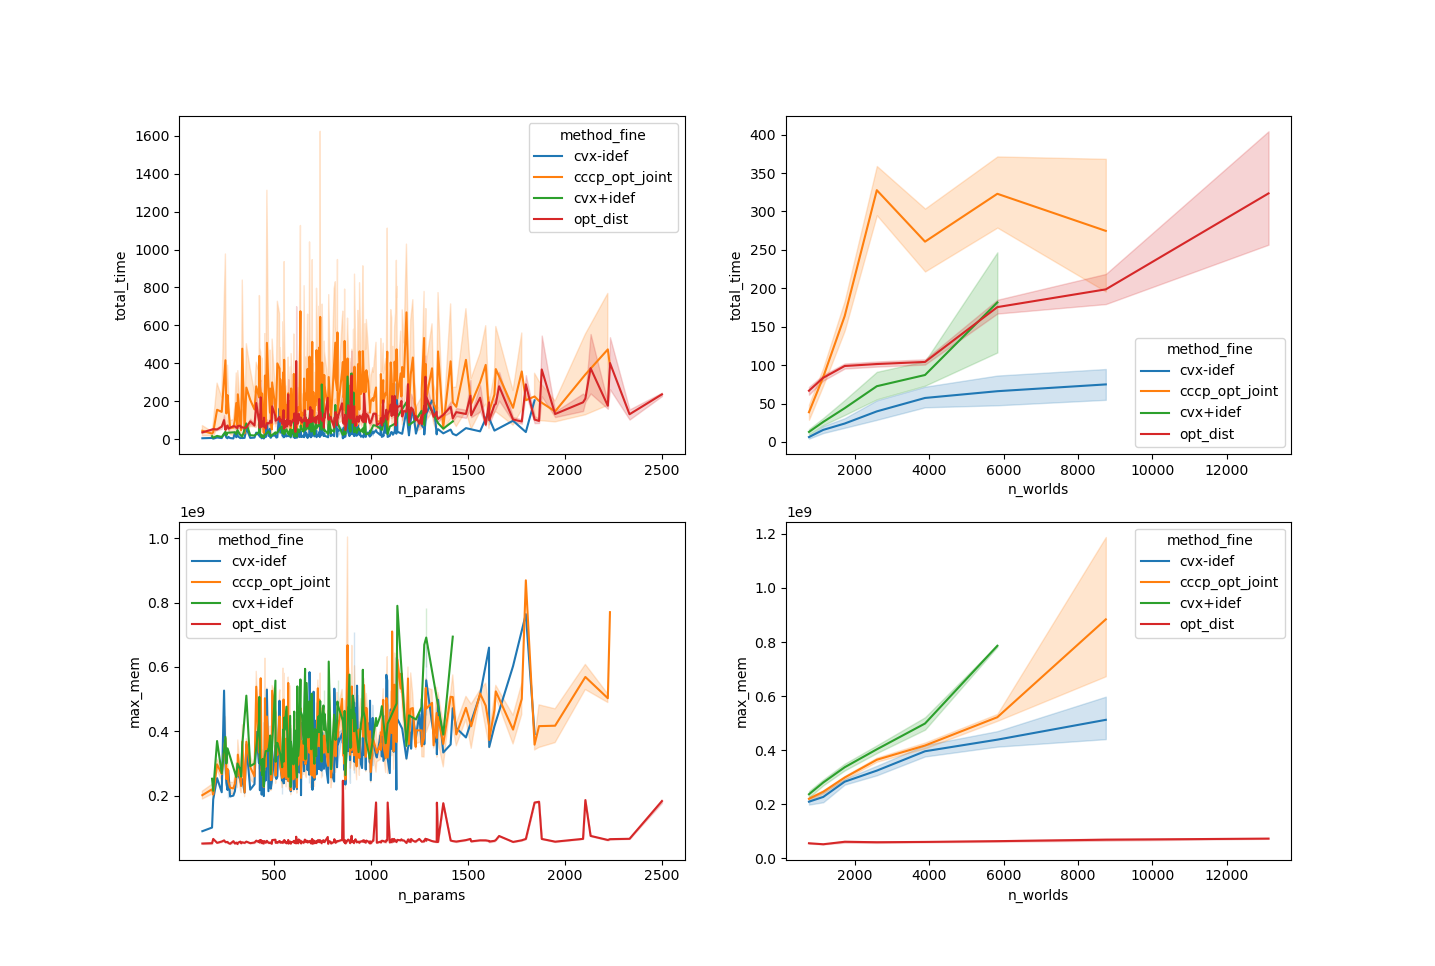
\includegraphics[width=\linewidth]{figs/resources-fine}
    \caption{
        The amount of resources: computation time (top) and maximum memory usage (bottom) for the various optimization methods (by color), as the size of the PDG increases, as measured by \texttt{n\_worlds} (right) and \texttt{n\_params} (left).
     }\label{fig:resources}
\end{figure}

\begin{figure}
    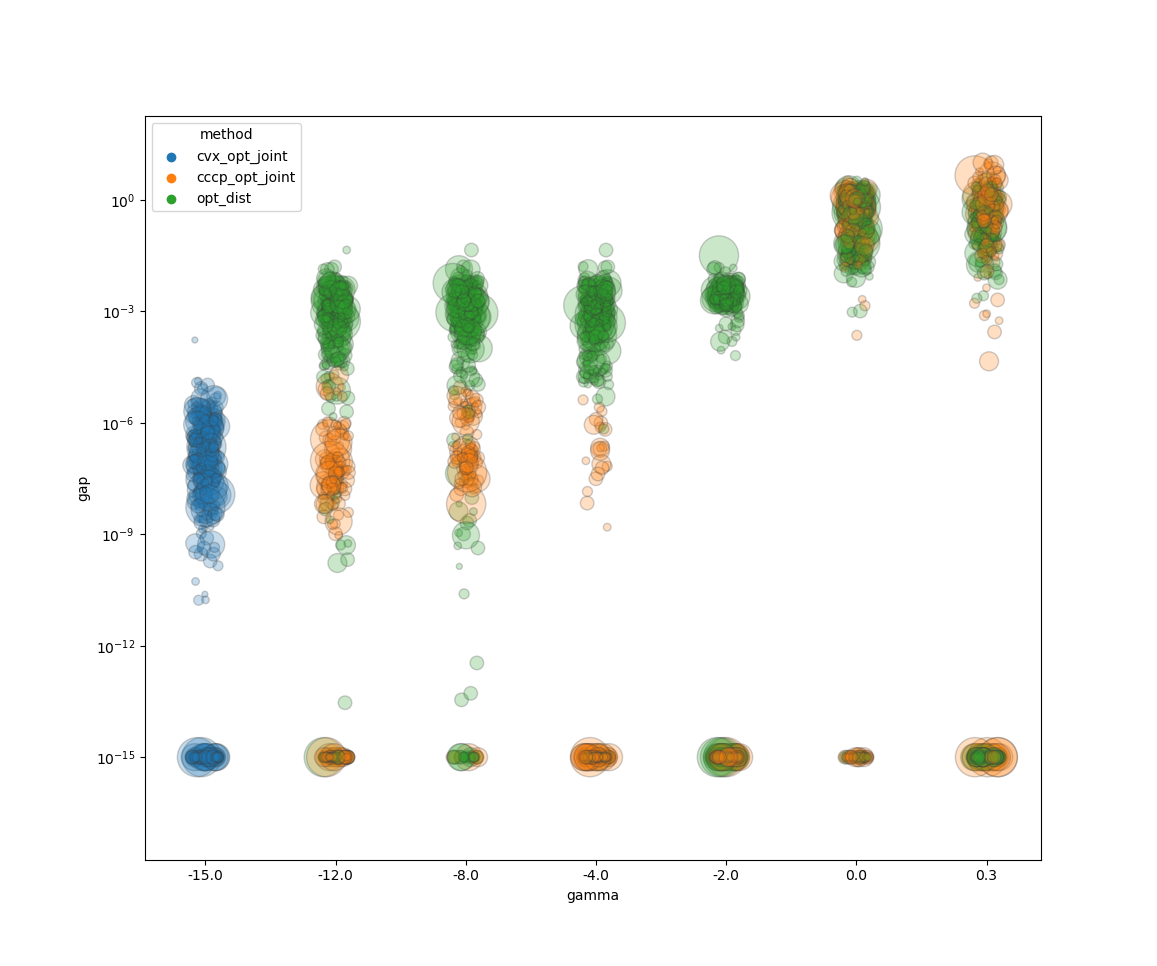
\includegraphics[width=\linewidth]{figs/gamma-vs-gap-bettergap}
    \caption{
        A graph of the gap (the difference between the attained objective value, and the best objective value obtained across all methods for that value of $\gamma$),
        as $\gamma$ varies. As before, colors indicate method.
        The size of the circle illustrates the relative number of worlds.
    }\label{fig:gamma-v-gap}
\end{figure}


\begin{figure}
    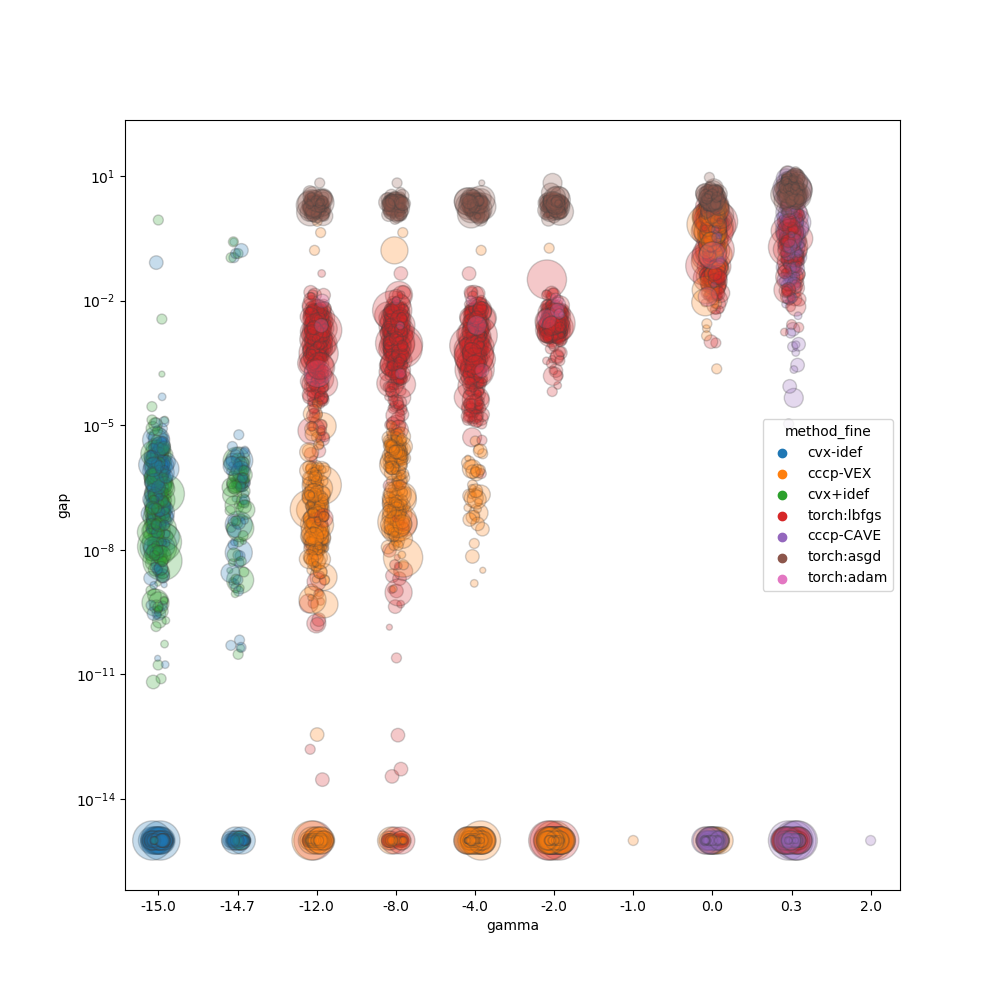
\includegraphics[width=\linewidth]{figs/2}
    \caption{
        A fine-grained variant of \cref{fig:gamma-v-gap}, which splits each method into sub-groups.
        The ExpCone methods \texttt{cvx\_opt\_joint} are split into two variants, depending on whether or not it also computed the second step described in \cref{sec:also-idef} to account for $\IDef{}$.
        The CCCP variants are \texttt{cccp\_opt\_joint} split into regimes where the entire problem is convex, and the entire problem is concave. The optimization approaches \texttt{opt\_dist} are split into three different optimizers: LBFGS, Adam, and accelerated Gradient Descent.
    }\label{fig:gamma-v-gap-fine}
\end{figure}

\begin{figure}
    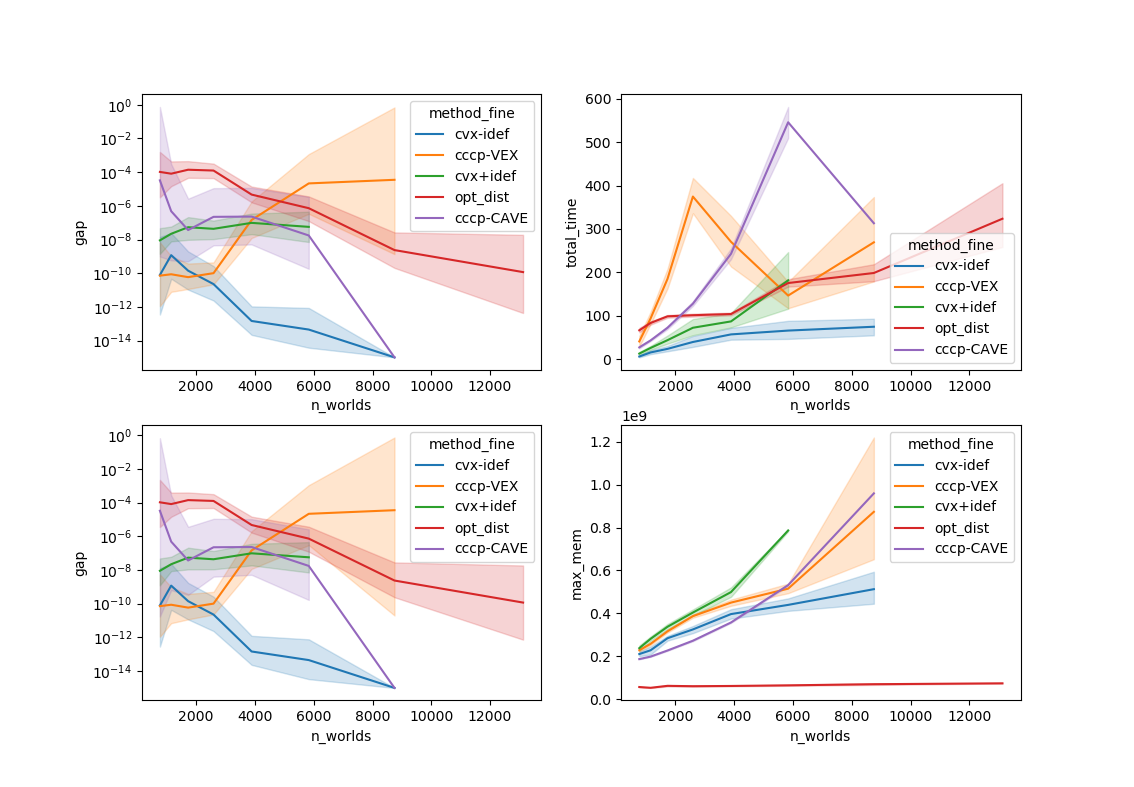
\includegraphics[width=\linewidth]{figs/1}
    \caption{
        A fine-grained variant of the right half of \cref{fig:resources},
        with gap information on the left.
    }\label{fig:gap-resource-fine}
\end{figure}


\begin{figure}
    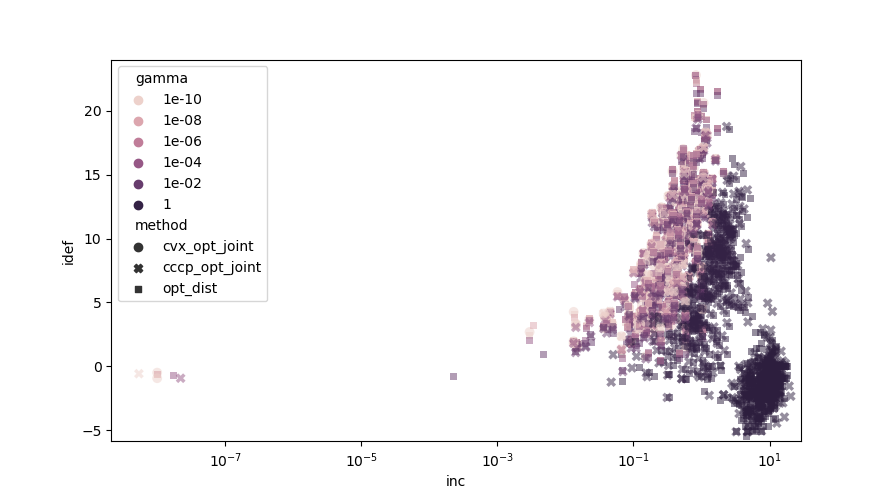
\includegraphics[width=\linewidth]{figs/inc-idef2}
    \caption{An illustration of the trade-off between $\Inc$ and $\IDef{}$. Darker collors correspond to larger $\gamma$.}\label{fig:inc-idef}
\end{figure}

\subsection{Comparison To Belief propagation}

Since PDGs generalize other graphical models, one might wonder how our method stacks up against them.
We benchmarked against the small networks, and some of the medium-sized ones, from the \href{https://www.bnlearn.com/bnrepository/}{\texttt{bnlearn}} repository.



\subsection{Evaluations On Random PDGSs}
We start by focusing on empirical properties of the optimization over joint distributions.

We generated several hundred PDGs with various properties: 9 or 10 variables, each of which can take 2-3 values. Each PDG contains 7-15 hyperedges, with 1-2 target nodes and 0-3 source nodes. The cpds are chosen by taking uniformly random numbers from [0,1] and normalizing appropriately, and every $\beta$ is set to 1.
For each PDG $\dg M$, we measure its complexity by:
\begin{itemize}[nosep]
    \item \texttt{n\_edges}, the number of edges in $\dg M$,
    \item \texttt{n\_params}, the total number of parameters across all the cpds of $\dg M$, and
    \item \texttt{n\_worlds}, the size of the joint distributions on the variables of $\dg M$.
\end{itemize}

\textbf{Capacity.}
The black-box py-torch based approaches clearly have an edge in that they can handle larger models; see the cut-offs on the right sides of \cref{fig:resources,fig:gap-resource-fine}.

\textbf{Resource Costs.}
Look at \cref{fig:resources}.
Note that the exponential cone methods without the CCCP (blue and green) are actually faster than LBFGS, which was the best-performing torch optimizer.
However, they use \emph{significantly} more memory, and cannot handle more than 8000 worlds.


\textbf{Accuracy.}
In addition to being faster, the exponential cone techniques are also more preicse.
Note that the CCCP is typically more precise than the black-box optimizers when the problem is fully convex $\gamma \le 1$, and mirrors the performance of the exp-cone algorithms for the quantitative limit on the left, in blue.  For combinations of larger $\gamma$ and more worlds however, the 20 iteration maximum we imposed is not nearly enough to get convergence, and the black-box optimizers are both faster and attain better objective values.

\section{DISCUSSION}

% Our anaysis
Our analysis shows that inference in PDGs with bounded tree-width can be done .


\TODO[ the below is a transplant without context; fix it ]
% % Some queries are more difficult than others.
% Although we the question the same way, we also want to point out that there are other reasonable ways to answer that question once we move to PDGs.
% Suppose we were looking at a BN in which it just so happens that $\mat X$ contains only a single variable and $\mat Y$ are the parents of $\mat X$.
% In this case, our representation already contains the probabilities we are looking for, and we would be happy returning that row of the conditional probability table.
% But in a PDG, that cpd $p(\mat Y \,|\,\mat X)$, even if it is the only one
% attached to an edge from $X$ to $Y$, may not be the same as $\bbr{\dg M}^*(Y|X)$.
% As a consequence,




\subsubsection*{Acknowledgements}
% All acknowledgments go at the end of the paper, including thanks to reviewers who gave useful comments, to colleagues who contributed to the ideas, and to funding agencies and corporate sponsors that provided financial support.
% To preserve the anonymity, please include acknowledgments \emph{only} in the camera-ready papers.

\subsubsection*{References}
\printbibliography


\clearpage
\onecolumn
\appendix
\section{Proofs}

\recall{theorem:main}
\begin{lproof}\label{proof:main}
    We apply the analysis of \textcite{badenbroek2021algorithm}.
    The primal conic problem
    \[
        \inf_{x} \{\langle c, x\rangle : Ax = b, x \in K \tag{D}
    \]

\end{lproof}

\subsection{}

\recall{prop:smooth-and-strictly-cvx}
\begin{lproof}\label{proof:smooth-and-strictly-cvx}
	% First, we deal with the convexity, for which we make use of \cref{lem:cvx2}.
	% \commentout{
	% 	\def\mw#1{{\mat w}_{\!_{#1}}}
	% 	\def\ofmw(#1|#2){(\mw{#1} | \mw{#2})}
	% 	\begin{align*}
	% 		\aar{\dg M \bundle p}_\gamma &= \inf_\mu \Big[ \Inc_{\dg M \bundle p}(\mu)
	% 			+ \IDef{\dg M \bundle p}(\mu) \Big] \\
	% 		&=  \inf_{\mu} \Ex_{\mat w \sim \mu}
	% 			\left[\log \mu(\mat w) +
	% 			 	\beta_p \log \frac{\mu\ofmw(Y|X)}{p\ofmw(Y|X)} \; +  \!\sum_{\ed LAB} \beta_L \log \frac{\mu\ofmw(B|A)}{\bp\ofmw(B|A)} + \alpha_L \log \frac{0}{\mu\ofmw(B|A)}\right] \\
	% 		&= f
	% 	\end{align*}
	% }
	We start by expanding the definitions, obtaining
	\begin{align*}
		\aar{\dg M \bundle p}_\gamma &= \inf_\mu ~\bbr{\dg M \bundle p}_\gamma(\mu) \\
			&= \inf_\mu \left[ \bbr{\dg M }_\gamma(\mu)
				+ \Ex_{x\sim\mu_{\!_X}} \kldiv[\Big]{\mu(Y\mid x)}{p(Y\mid x)} \right]\\
			&= \inf_\mu \left[ \bbr{\dg M }_\gamma(\mu)
				+  \kldiv[\Big]{\mu(X,Y)}{p(Y \mid X)\, \mu(X)} \right].
	\end{align*}
	% % Choose $\gamma < \min (\{1\}\cup\{ \beta^{\dg M}_L : L \in \Ed^{\dg M}\})$.
	% Since $\bbr{\dg M}_\gamma$ is a $\gamma$-strongly convex function of $\mu$ for all
	% such $\gamma < \min_L \beta_L$, and
	% $\kldiv{\mu_{XY}}{\mu_X \; p_{Y\mid X}}$ is 1-strongly
	% convex in $p$ for fixed $\mu$ (\cref{lem:Dstrongcvx}),
	% % $\thickD$ is convex in both of its arguments,
	% their sum is $\gamma$-strongly convex in $\mu$ and in $p$.
	% By \cref{lem:cvx2} taking an infemum preserves this convexity,
	% and so
	% $
	%  	\inf_\mu \left[ \bbr{\dg M }_\gamma(\mu)
	% 	+  \kldiv[\big]{\mu_{XY}}{p_{Y \mid X}\; \mu_X} \right]
	% $, which equals $\aar{\dg M \bundle p}_\gamma$,
	% is $\gamma$-strongly convex in $p$.
	% % $\aar{\dg M \bundle p}_\gamma$ is smooth
	% % Smoothness.


	% Choose $\gamma < \min (\{1\}\cup\{ \beta^{\dg M}_L : L \in \Ed^{\dg M}\})$.
	Fix $\gamma < \min_L \beta_L$. Then we know that $\bbr{\dg X}_\gamma(\mu)$ is a $\gamma$-strongly convex function for every PDG $\dg X$, and hence there is a unique joint distribution which minimizes it.

	\textbf{Strict Convexity.}
	Suppose $p_1(Y \mid X)$ and $p_2(Y\mid X)$ are two cpds on $Y$ given $X$.
	Fix $\lambda \in [0,1]$, and set $p_\lambda = (1-\lambda) p_1 + \lambda p_2$.
	Let $\mu_1, \mu_2$ and $\mu_\lambda$ be the joint distributions that minimze $\bbr{\dg M \bundle p_1}_\gamma$, $\bbr{\dg M \bundle p_2}_\gamma$ and $\bbr{\dg M \bundle p_\lambda}_\gamma$, respectively.  Then we have
	\begin{equation*}
		\aar{\dg M \bundle p_\lambda}_\gamma
			= \bbr{\dg M}_\gamma(\mu_\lambda) + \kldiv[\Big]{\mu_\lambda(X,Y)}{p_\lambda(Y\mid X) \mu_\lambda( X)}.
	\end{equation*}
	By convexity of $\bbr{\dg M}$ and $\thickD$, we have
	\begin{align}
		\bbr{\dg M}_\gamma(\mu_\lambda)
		 	&\le (\lambda-1)\bbr{\dg M}_\gamma(\mu_1) + \lambda \bbr{\dg M}_\gamma(\mu_2)
			 	\label{eqn:score-cvx}\\
		\text{and}\qquad \kldiv[\Big]{\mu_\lambda(XY)}{p_\lambda(Y | X) \mu_\lambda( X)}
			&\le (1-\lambda)\kldiv[\Big]{\mu_1(XY)}{p_1(Y | X) \mu_1( X)} \nonumber \\
			&\qquad+ \lambda\;\;\kldiv[\Big]{\mu_2(XY)}{p_2(Y | X) \mu_2( X)}.
				\label{eqn:D-cvx}
	\end{align}
	If $\mu_1 \ne \mu_2$ then since $\bbr{\dg M}$ is strictly convex, \eqref{eqn:score-cvx} must
	be a strict inequality. On the other hand, if $\mu_1 = \mu_2$, then since $\mu_\lambda = \mu_1 = \mu_2$ and $\thickD$ is stricly convex in its second argument when its first argument is fixed (\Cref{lem:Dstrongcvx}), \eqref{eqn:D-cvx} must be a strict inequality.
	In either case, the sum of the two inequalities must be strict, giving us
	\begin{align*}
		\aar{\dg M \bundle p_\lambda}_\gamma &=
		\bbr{\dg M}_\gamma(\mu_\lambda) + \kldiv[\Big]{\mu_\lambda(XY)}{p_\lambda(Y | X) \mu_\lambda( X)} \\
		&<
		 (\lambda-1) \left[\bbr{\dg M}_\gamma(\mu_1)
			 	+ \kldiv[\Big]{\mu_1(XY)}{p_1(Y | X) \mu_1( X)} \right]
			 \\[-0.3em]&\qquad\qquad
			 + \lambda \left[ \bbr{\dg M}_\gamma(\mu_2)
			 	+ \kldiv[\Big]{\mu_2(XY)}{p_2(Y | X) \mu_2( X)}
			 	\right] \\
		 &= (\lambda-1) \aar{\dg M \bundle p_1} + \lambda\,\aar{\dg M \bundle p_2},
	\end{align*}
	which shows that $\aar{\dg M \bundle p}$ is \emph{strictly} convex in $p$, as desired.


	\textbf{Smoothness.}
	If $\bbr{\dg M \bundle p}_\gamma^*$ is a positive distribution, then by definition $\bbr{\dg M \bundle p}$ achieves its minimum on the interior of the probability simplex $\Delta \V(\dg M \bundle p)$, and so by \Cref{lem:cvx4}, we immediately find that $\aar{\dg M \bundle p}_\gamma$ is smooth in $p$.

	Now, suppose that $\bbr{\dg M \bundle p}_\gamma^*(\mat w) = 0$,  for some $\mat w \in \V(\dg M \bundle p)$.

	Applying \Cref{lem:cvx4} to the function $f = \bbr{\dg M}_\gamma$

	Now for the second case.

	\TODO

	If $x^*_b \in \partial X$, then we claim that either
	\begin{enumerate}[nosep]
		\item There is a subspace $T \subseteq \mathbb R^{m}$ with
			$\SD{}$
	 	\item There is a subspace $S \subseteq \mathbb R^{n}$ with
			$x^*_b \in S \cap \partial X$ such

	\end{enumerate}

\end{lproof}

\begin{lemma}\label{lem:cvx4}
	Let $X$ and $Y$ be convex sets, and
	$f : X \times Y \to \mathbb R$ be a smooth $(C^\infty)$, convex function.
	If $f$ is strictly convex in $X$, and for some $y_0 \in Y$, $f(x, y_0)$ achieves its infemum on the interior of $X$.
	then $y\mapsto \inf_x f(x, y)$ is smooth $(C^\infty)$ at the point $y_0$.
\end{lemma}

\begin{lproof}%[Proof of \Cref{lem:cvx4}]
	% Let $f_y(x) = f(x,y)$.
	% Since $f$ is smooth and stritly convex, each restriction $f_y$ of $f$ to a
	% particular $y$ is also smooth and strictly convex.
	% As a result, each $f_y$ has a unique minimum $m_y := \inf_{x} f_y(x)$.
	% As $f_y$ is smooth, $m_y$ is either a boundary point, or
	% at a point where $\nabla f_y = 0$.
	%
	% Moreover, it is a constrained optimization problem, so
	% $\nabla_{x,y,\lambda} [ f(x,y) + \lambda (y_0 - y)] = 0$.
	%
	% \TODO
	Let $x_0^* := \arg\min_x f(x,y_0)$, which is achieved by assumption, and is unique because $f(-,y_0)$ is strictly convex.

	We will ultimately apply the implicit function theorem to give us a smooth function which is equal to this infemum, but to do so we must deal with the technicality that it requires an open set; the boundary is the most complicated part of this result.
	Here we have essentially required that the domain be open by fiat for $X$, but for $Y$ (which is a possibly non-open subset of $\mathbb R^m$), we use the Extension Lemma for smooth functions \cite[Lemma 2.26]{Lee.SmoothManifolds}. In our context, it states that
	for every open set $U$ with $\overline{Y} \subseteq U \subseteq \mathbb R^m$,
	there exists a function $\tilde f : X \times \mathbb R^m \to \mathbb R$, such that $\tilde f |_{Y} = f$ (and $\supp \tilde f \subseteq U$).
	We only need a small fraction of this power: that we can smoothly extend $f$ to \emph{some} open set of $\mathbb R^m$, which we fix and call $\tilde Y$.

	% Similarly, for other $y \in Y$, let $x^*_y$ be the unique value of $x$ which minimizes $f(x,y)$.

	% \textbf{Smoothness.}
	% By assumption, $x^*_b$ is not a boundary point of $X$.
	%
	We claim that now all conditions for the Implicit Function Theorem are met if invoked with
		$\phi(y,x) := \vec\nabla_x \tilde f(x,y)$ and $(\mat b,\mat a) = (y_0, x^*_0)$.
	Concretely, we have $m = \mathop{dim} X$, $n = \mathop{dim} Y$, and $Z = (\tilde Y \times X)^\circ$, i.e., the interior of $\tilde Y \times X$, which is open and contains $(\mat b, \mat a)$.
	 Becuase $\phi$ is smooth, it is $k$-times differentiable for all $k$. We have $\vec\nabla_x \tilde f (y_0, x^*_0) = \vec 0$ because $x^*_0$ is a local minimum of the smooth function $\tilde f(-, y_0)$ which lies on the interior of $X$.

	Moreover, the Jacobian matrix
	\[ \mat J_{\nabla\!\tilde f, x}(y_0, x_0^*) = \left[ \frac{\partial^2 f}{\partial x_i \partial x_j}(x^*_0, y_0) \right]\]
	is the Hessian of the strictly convex funtion $f(-, b)$, and therefore positive definite (and in particular non-singular).
	Therefore, the Implicit Function Theorem guarantees us the existence of a neighborhood $U \subset \tilde Y$ of $y_0$ for which
	there is a unique $k$-times differentiable function $g: U \to X$ such that $g(y_0) = x^*_0$ and $\vec\nabla_x \tilde f(y, g(y)) = 0$ for all $y \in U$. Of course, this implies $g(y) = \argmin_x f(x,y)$ at every such point, and $\inf_x f(x,y) = f(g(y),y)$ is a composition of the smooth function $f$ with the $k$-times differentiable function $g \otimes \mathrm{id}_Y$.
	Therefore, $\inf_x f(x,y)$ is itself $k$-times continuously differentiable at $y_0$ for all $k$, or in other words, $\inf_x f(x,y)$ is smooth at $y=y_0$.
\end{lproof}

\recall{prop:markov-property}
\begin{lproof}
	Choose $\mu \in \bbr{\dg M_1 \bundle \dg M_2}^*_\gamma$.
	% Choose $\mu \in \mu^*_\gamma (\dg M_1 \bundle \dg M_2)$.
	Let $\mu' := \mu(\X_1) \mu(\X_2)$

	\TODO[Finish Transcribing Proof]
\end{lproof}


\subsection{Hardness Results}

\recall{prop:consistent-NP-hard}
\begin{lproof} \label{proof:consistent-NP-hard}
	We can directly encode SAT problems as PDGs.
	Specifically, let
	$$\varphi := \bigwedge_{j \in \mathcal J} \bigvee_{i \in \mathcal I(j)} (X_{j,i})$$
	be a CNF formula over binary variables $\mat X := \bigcup_{j,i} X_{j,i}$. Let
	$\dg M_\varphi$ be the PDG containing every variable $X \in \mat X$ and a binary
	variable $C_j$ (taking the value 0 or 1) for each clause $j \in \mathcal J$, as well as the following edges, for each $j \in \mathcal J$:
	%\{$``$\varphi(\mat X)$''$\}$ with $\V(\varphi) = \{0,1\}$, and
	\begin{itemize}
		\item a hyperedge $\{X_{j,i} : i \in \mathcal I(j)\} \tto C_j$, together with a degenerate cpd
			encoding the boolean OR function (i.e., the truth of $C_j$ given $\{X_{j,i}\}$);
		\item an edge $\pdgunit \tto C_j$, together with a cpd asserting $C_j$ be equal to 1.
	\end{itemize}
	% We give each edge $\alpha = 0$ and $\beta = 1$.
	First, note that the number of nodes, edges, and non-zero entries in the cpds are polynomial in the $|\mathcal J|, |\mat X|$, and the total number of parameters in a simple matrix representation of the cpds is also polynomial if $\mathcal I$ is bounded (e.g., if $\varphi$ is a 3-CNF formula).
	A satisfying assignment $\mat x \models \varphi$ of the variables $\mat X$ can be regarded as a degenerate joint distribution $\delta_{\mat X = \mat x}$ on $\mat X$, and extends uniquely to a full joint distribution $\mu_{\mat x} \in \Delta \V(\dg M_\varphi)$ consistent with all of the edges, by
	\[ \mu_{\mat x} = \delta_{\mat x} \otimes \delta_{\{C_j = \vee_i  x_{j,i}\}} \]

 	Conversely, if $\mu$ is a joint distribution consistent with the edges above, then any point $\mat x$ in the support of $\mu(\mat X)$ must be a satisfying assignment, since the two classes of edges respectively ensure that $1 =\mu(C_j\!=\! 1 \mid \mat X \!=\! \mat x) = \bigvee_{i \in \mathcal I(j)} \mat x_{j,i}$ for all $j \in \mathcal J$, and so $\mat x \models \varphi$.

	Thus, $\SD{\dg M_\varphi} \ne \emptyset$ if and only if $\varphi$ is satisfiable, so
	an algorithm for determining if a PDG is consistent can also be adapted (in polynomial space and time) for use as a SAT solver, and so the problem of determining if a PDG consistent is NP-hard.

% \end{lproof}
% \recall{prop:sharp-p-hard}
% \begin{lproof}\label{proof:sharp-p-hard}

    \medskip\hrule\smallskip

	\textbf{PART (b).}
    We prove this by reduction to \#SAT. Again, let $\varphi$ be some CNF formula over $\mat X$, and construct
	$\dg M_\varphi$ as in \hyperref[proof:consistent-NP-hard]{the proof} of
	\Cref{prop:consistent-NP-hard}.
	Furthemore, let $\bbr{\varphi} := \{ \mat x : \mat x \models \varphi \}$ be the set of  assingments to $\mat X$ satisfying $\varphi$, and $\#_\varphi := |\bbr{\dg M}|$ denote the number such assignments. We now claim that
	\begin{equation}\label{eqn:number-of-solns}
		\#_\varphi = \exp \left[- \frac1\gamma \aar{ \dg M_\varphi }_\gamma \right].
	\end{equation}
 	If true, we would have a reduced the \#P-hard problem of computing $\#_\varphi$ to the problem of computing $\aar{\dg M}_\gamma$ for fixed $\gamma$. We now proceed with proof \eqref{eqn:number-of-solns}.
	By definition, we have
	\[ \aar{\dg M_\varphi}_\gamma = \inf_\mu \Big[ \Inc_{\dg M_\varphi}(\mu) + \gamma \IDef{\dg M_\varphi}(\mu) \Big]. \]
	We start with a claim about first term.
	% For the particular PDG $\dg M_\varphi$, the

	\begin{iclaim} \label{claim:separate-inc-varphi}
		% $\Inc(\dg M_\varphi)$ is finite if and only if $\varphi$ is statisfiable.
		$\Inc_{\dg M_\varphi}\!(\mu) =
		% \begin{cases}
		% 	0 & \text{if}~  \mat x \models \varphi~\text{and}~\mat c = \mat 1
		% 	 	~\text{for all}~(\mat x, \mat c) \in \supp \mu\\
		% 	\infty & \text{otherwise}
		% \end{cases}
		\begin{cases}
			0 & \text{if}~  \supp \mu \subseteq \bbr{\varphi} \times \{ \mat 1\} \\
			\infty & \text{otherwise}
		\end{cases}$.
	\end{iclaim}
	\vspace{-1em}
	\begin{lproof}
		Writing out the definition explicitly, the first can be written as
		\begin{equation}
			\Inc_{\dg M_\varphi}\!(\mu) = \sum_{j} \left[ \kldiv[\Big]{\mu(C_j)}{\delta_1} +
				\Ex_{\mat x \sim \mu(\mat X_j)} \kldiv[\Big]{\mu(C_j \mid \mat X_j = \mat x)}{\delta_{\lor_i \mat x_{j,i}}} \right], \label{eqn:explicit-INC-Mvarphi}
				% &= \sum_{j} \left[
				% 	\begin{matrix} \mu(C_j\!=\!0) (\infty) \\
				% 	 	+ \mu(C_j \!=\! 1) \log \mu(C_j \!=\! 1)
				% 	\end{matrix} +
				% 	\Ex_{\mat x \sim \mu(\mat X_j)} \kldiv[\Big]{\mu(C_j \mid \mat X_j = \mat x)}{\delta_{\lor_i \mat x_i}} \right],
		\end{equation}
		where $\mat X_j = \{X_{ij} : j \in \mathcal I(j)\}$ is the set of variables that
		appear in clause $j$, and $\delta_{(-)}$ is the probability distribution placing all mass on the point indicated by its subscript.
		As a reminder, the relative entropy is given by
		\[ \kldiv[\Big]{\mu(\Omega)}{\nu(\Omega)} := \Ex_{\omega \sim \mu} \log \frac{\mu(\omega)}{\nu(\omega)},
		\quad\parbox{1.4in}{\centering and in particular, \\ if $\Omega$ is binary,}\quad
			\kldiv[\big]{\mu(\Omega)}{\delta_\omega} = \begin{cases}
				0 &  \text{if}~\mu(\omega) = 1 ; \\
				\infty & \text{otherwise}.
		\end{cases} \]
		Applying this to \eqref{eqn:explicit-INC-Mvarphi}, we find that either:
		\begin{enumerate}[itemsep=0pt]
			\item Every term of \eqref{eqn:explicit-INC-Mvarphi} is finite (and zero) so $\Inc_{\dg M_\varphi}(\mu) = 0$, which happens when $\mu(C_j = 1) = 1$ and $\mu(C_j = \vee_i~ x_{j,i}) = 1$ for all $j$.  In this case, $\mat c = \mat 1 = \{ \vee_i~x_{j,i} \}_j$ so $\mat x \models \varphi$ for every $(\mat{c,x}) \in \supp \mu$;
			\item Some term of \eqref{eqn:explicit-INC-Mvarphi} is infinite, so that $\Inc_{\dg M_\varphi}(\mu) = \infty$, which happens if some $j$, either

			\begin{enumerate}
				\item $\mu(C_j \ne 1) > 0$ --- in which case there is some $(\mat{x,c}) \in \supp \mu$ with $\mat c \ne 1$, or
				\item $\supp \mu(\mat C) = \{\mat 1\}$, but $\mu(C_j \ne \vee_i~ x_{j,i}) > 0$ --- in which case there is some $(\mat{x,1}) \in \supp \mu$ for which $1 = c_j \ne \vee_i~x_{j,i}\;$, and so $\mat x \not\models \varphi$.
			\end{enumerate}
		\end{enumerate}
		Condensing and rearranging slightly, we have shown that
		\[
			\Inc_{\dg M_\varphi}(\mu) =
			\begin{cases}
				0 & \text{if}~  \mat x \models \varphi~\text{and}~\mat c = \mat 1
				 	~\text{for all}~(\mat x, \mat c) \in \supp \mu\\
				\infty & \text{otherwise}
			\end{cases}~.
		\]
		% So if $\mat x \models \varphi$ for all $\mat x \in \supp \mu(X)$,
		%
		% $\Inc_{\dg M_\varphi}(\mu) = 0$
		% The first term is infinite if $\mu(C_j = 1) < 1$, and the second is infinite
		% if $\mu(C_j = \lor_i X_{i,j}) < 1$. Thus, if $\Inc_{\dg M_\varphi}(\mu)$ is finite, then $\mat x \sim \mu(\mat X)$ satisfies $\varphi$ with probability 1, and $\varphi$ must be satisfiable.
		% Conversely,
	\end{lproof}

	% Thus, if $\Inc_{\dg M_\varphi}(\mu)$ is finite, then every $\mat x \in \supp \mu$ is a satisfying assignment of $\varphi$.
	Because $\IDef{}$ is bounded, it follows immediately that
 	$\aar{\dg M_\varphi}_\gamma$, is finite if and only if
	there is some distribution $\mu \in \Delta\V(\mat X,\mat C)$ for which $\Inc_{\dg M_\varphi}(\mu)$ is finite, or equivalently, by \Cref{claim:separate-inc-varphi}, iff there exists some $\mu(\mat X) \in \Delta \V(\mat X)$ for which $\supp \mu(\mat X) \subseteq \bbr{\varphi}$, which in turn is true if and only if $\varphi$ is satisfiable.

	In particular, if $\varphi$ is not satisfiable (i.e., $\#_\varphi = 0$), then $\aar{\dg M_\varphi}_\gamma = +\infty$, and
	\[
		\exp \left[ -\frac1\gamma \aar{\dg M_\varphi}_\gamma \right] =
	 		\exp [ - \infty ] = 0 = \#_\varphi,
	\]
	so in this case \eqref{eqn:number-of-solns} holds as promised. On the other hand, if $\varphi$ \emph{is} satisfiable, then, again by \Cref{claim:separate-inc-varphi}, every $\mu$ minimizing $\bbr{\dg M_\varphi}_\gamma$, (i.e., every $\mu \in \bbr{\dg M_\varphi}_\gamma^*$) must be supported entirely on $\bbr{\varphi}$ and have $\Inc_{\dg M_\varphi}\!(\mu) = 0$.  As a result, we have
	\[
		\aar{\dg M_\varphi}_\gamma =
			\inf\nolimits_{\mu \in \Delta \big[\bbr{\varphi} \times \{\mat 1\}\big]} \gamma\; \IDef{\dg M_\varphi}(\mu) .
	\]
	A priori, by the definition of $\IDef{\dg M_\varphi}$, we have
	\[
		\IDef{\dg M_\varphi}(\mu) =
		 	- \H(\mu) + \sum_{j} \Big[ \alpha_{j,1} \H_\mu(C_j \mid \mat X_j)
						+ \alpha_{j,0} \H_\mu(C_j) \Big],
	\]
	where $\alpha_{j,0}$ and $\alpha_{j,1}$ are values of $\alpha$ for the edges of $\dg M_\varphi$, which we have not specified because they are rendered irrelevant by the fact that their corresponding cpds are deterministic. We now show how this plays out in the present case.
	Any $\mu \in \Delta\big[\bbr{\varphi} \times \{\mat 1\}\big]$ we consider has a degenerate marginal on $\mat C$. Specifcally, for every $j$, we have $\mu(C_j) = \delta_1$, and since entropy is non-negative and never increased by conditioning,
	$$
		0 \le \H_\mu(C_j \mid \mat X_j) \le \H_\mu(C_j) = 0.
	$$
	Therefore, $\IDef{\dg M_\varphi}(\mu)$ reduces to the negative entropy of $\mu$.
	Finally, making use of the fact that the maximum entropy distribution $\mu^*$ supported on a finite set $S$ is the uniform distribution on $S$, and has $\H(\mu^*) = \log | S |$, we have
	\begin{align*}
		\aar{\dg M_\varphi}_\gamma &= \inf\nolimits_{\mu \in \Delta \big[\bbr{\varphi} \times \{\mat 1\}\big]} \gamma\; \IDef{\dg M_\varphi}(\mu) \\
			&= \inf\nolimits_{\mu \in \Delta \big[\bbr{\varphi} \times \{\mat 1\}\big]} -\, \gamma\, \H(\mu) \\
			&= - \gamma\, \sup\nolimits_{\mu \in \Delta \big[\bbr{\varphi} \times \{\mat 1\}\big]}  \H(\mu) \\
			&= - \gamma\, \log (\#_\varphi),
	\end{align*}
	\hspace{1in}giving us
	$$
		\#_\varphi = \exp \left[- \frac1\gamma \aar{ \dg M_\varphi }_\gamma \right],
	$$
	as desired. We have now reduced \#SAT to computing $\aar{\dg M}_\gamma$, for $\gamma \in \mathbb R^{>0}$ and an arbitrary PDG $\dg M$, which is therefore \#P-hard.
\end{lproof}



\section{INFERENCE VIA INCONSISTENCY MINIMIZATION}
    \label{sec:inf-via-inc}

We are now equipped to talk more technically about inference in PDGs.
% When working with traditional graphical models, the meaning is clear.
%k
Since PDG semantics are already given in terms of a scoring function,
% the obvious thing to do is to find a distribution that minimizes it.
the obvious thing to do is to find a distribution that minimizes it.
%joe2*: But what does this minimization have to do with the inference
%problem you defined above?
%oli2*: if you have a concrete joint distribution, computing marginal probabilities of it is trivial, and conditioning is not much harder. Did my additions help?
Such a distribution $\mu$ could straightforwardly be used to answer probabilistic queries \eqref{q:inf} and compute inconsistency.
% There are several immediate difficulties.
There are some immediate difficulties with this approach.
% We immediately run into some obstacles.
% There are some obstacles to this.


\begin{enumerate}[nosep, label=\textbf{D\arabic*.}]
    \item Even writing down a distribution $\mu$, let alone evaluating its score $\bbr{\dg M}_\gamma (\mu)$, or minimizing it, takes exponential time.

    \item Generally speaking, optimization is computationally difficult.
        Even our most powerful optimization techniques only provably find optima in certain special cases.
    Unfortunately, while standard optimization techniques seem to work in practice
%joe1: why don't the standard tools apply in our setting?
%oli1: the next sentence explains it: the standard tools require Lipshitz-ness or
% self-concordance. How can I write this more clearly, if I don't really want to go into
% either but still want to mention the names so that people know what doesn't work?
%  (actually, the way the optimizer works is by using a self-concordant barrier function,
%       which is realted, but we can't use self-concordance directly in the obvious way.)
%
%      (more-or-less; see \cref{sec:expts}), the standard theoretical
      (more or less; see \cref{sec:expts}), the standard theoretical
      tools do not apply in our setting.
        % and even if it can be
%joe2*: What does it even mean for a pdg to be strictly convex?
%oli2*: The scoring function is convex, in its argument $\mu$. Is this unclear from the wording? [[M]]_\gamma is the scoring function.
%oli2: adding wording to try to abdicate responsibility for motivation
        % Despite being strictly convex,
        To be technical: despite being strictly convex,
        %oli2: removing because I have too many duplicate citations.
        % \parencite[at least for small $\gamma$,][]{pdg-aaai},
        and even $C^\infty$ smooth,
%joe1: I have no idea what self-concordant means.  Unless you're sure
%that over 90% of AIStats folks will now, you must define it and
%explain why it's relevant.  At least I know what the Lipshitz
%condition is, but it couldn't hurt to explain that too.
%joe2*: You still need to explain these terms and MOTIVATE why we care
%about them.
%oli2: I don't really. I want this to be a passing remark for those who know about self-concordance (which I'd guess is 40% of AISTATS folks) and Lipshitz-ness (I'd guess > 95% of AISTATS), but I really don't wan't to make a big deal of either of these two things. They're not important to me, they're just the standard tools that I don't think work. What do you think I should do?
        in general $\bbr{\dg M}_\gamma$ seems to be neither Lipshitz nor self-concordant.
         % convex (in $\mu$, which is exponentially large),
    \item Even if we coulld easily find optimizers of the function $\bbr{\dg M}_\gamma$ for fixed $\gamma > 0$, it's still not obvious that this would allow us to calculate the unique limiting distribution $\bbr{\dg M}^*$.
\end{enumerate}

We will ultimately address each of these issues, but before we do so,
% let's start with a shift in perspective.
let's start by trying to do inference as
suggested in the final section of \textcite{pdg-aaai}, which meshes well with
the persepctive taken in \textcite{one-true-loss}.

%joe2*: As I said, this should already be in the intro
%oli2*: As I responded below with %oli1, I disagree because it doesn't pan out;
% it's just an interesting perspective. I think this is the right place for it.
The argument there is that one can do modeling as follows:
    represent all of the relevant information as cpds,
    form a PDG out of them, and
%joe2*: I'm lost.  What knobs do we have?  This comes out of the blue.
%oli2: in this case, just $p(Y|X)$, but I was trying to reerence the general approach
% of my first AISTATS paper, not talk about this in particular. I've done a minor
% tweak to the wording to try to make this clear.
    % play with the knobs you have to to minimize the resulting inconsistency.
    play with whatever knobs are available, so as to minimize the overall inconsistency.
% Well, we have a PDG $\dg M$, and we also have a candidate joint distribution $\mu$.
% What if we put them both on the same footing, in a new PDG, and measure its inconsistency?
%joe1
%It is not hard to show that the distribution any distribution $\mu$
%that minimizes this quantity must also satisfy $\mu \in \bbr{\dg
% It is not hard to show that any distribution
% that minimizes this quantity must be in $\bbr{\dg
  % M}_\gamma^*$. More generally,
Well, we have a PDG $\dg M$, and we wanted to know the probablility of $Y$ given $X$.
What happens if we extend $\dg M$ with a guess, say $p(Y|X)$, and then
%oli2: added, to address your concern below
alter $p$ so as to minimize inconsistency?
As hinted in \textcite{pdg-aaai},
this
%oli2: modified
% would indeed perform our inference task,
would indeed suffice for inference,
%oli2: also added
since the optimal value of $p(Y|X)$ would be the cpd we wanted.

%joe2*: What does this proposition have to  say about the inference
%task you defined earlier.  A priori, it doesn't look that closely related.
%oli2: did my additions above help?
\begin{linked}{prop}{optimalYgivenX}
	% \label{prop:optimalYgivenX}
	% For all $\dg M$, $X,Y\in\X^{\dg M}$, and $\gamma > 0$, we have that
    For all variables $X,Y$, and $\gamma > 0$,
	$$\displaystyle
		% \argmin_{p : X \to \Delta Y}
		\argmin_{p(Y|X)}\,
        \aar{\dg M + p}_\gamma =
		\Big\{ \mu(Y | X) :  \mu \in \bbr{\dg M}_\gamma^* \Big\}
	,$$
% \end{linked}
%
% In the limit of small $\gamma$, since there is only one such distribution,
% the expression beomes simpler.
%
% \begin{linked}{coro}{smallgammaopt}
%joe1: What's a "quantiative limit"?
%oli1: it's the limit as \gamma -> 0;
% I defined it when I defined [[M]]^*, and also it's not necessary
% to remember the worlds, because the symbols are sufficient to get the meaning.
and in the quantiative limit,
	$\displaystyle
		\bbr{\dg M}^*(Y | X)
	$ is the unique minimizer of the function
$
    p(Y|X) \mapsto \aar{\dg M + p}
$
% which  a conditional probability on $Y$ given $X$ into the PDG $\dg M$.
%joe1: I have no idea what you're trying to say here.  What does it
%mean that it "includes a conditional probability on $Y$ given $X$
%into the PDG"
%oli1: good point--- I'm not just adding ("includig") the new probability, but
% also measuring its inconsistency.
% which measures the inconsistency of
\end{linked}

%joe1*: The claim that we can use inconsistency to compute the
%marginal probability of somne (small) set of variables is an
%important part of the story of why inconsistency is important, and
%should have come *much* earlier (i.e., in the introduction)
%
%oli1: If this was what gave the reason we don't discuss it in the introduction
Consequently, if we are interested only in querying the marginal probability of some small subset $Y$ of variables conditioned on other ones $X$ (i.e., the usual form of a query to a graphical model), and we had an efficient way to estimate the inconsistency of a guess $p(Y|X)$ with the rest of the model, we would have successfully cleared obstacle \textbf{D1}.

% Since inference in other graphical models is already NP-hard,
% and the class of PDGs subsumes capture them, it should be no surprise
% that inference in PDGs is NP hard as well.
%
%
% One might imagine that \emph{resolving} the inconsistency is the hard part,
%     as opposed to noticing it.
% Might it easier to simply determine whether or not a PDG is inconsistent?

Since inference in other graphical models is already NP-hard,
and PDGs subsume them, it should come as no surprise
that inference in PDGs is NP hard as well.
%
Still, one might imagine that \emph{resolving} the inconsistency is the hard part,
    as opposed to noticing it.
Might it easier to simply determine whether or not a PDG is inconsistent?
% If this seems reasonable, you might suspect that this reformulation could increase the difficulty of optimization (\textbf{D2})---that we might lose the several nice properties we do have (strict convexity and smoothness)---but this concern turns out not to be substantiated.
%
%joe2: we don't need to try to get into the reader's head
%oli2: the problem is that it doesn't (clearly) increase the difficulty of the optimization, so "this could increase" is wrong. I only mean to suggest that one might suspect that.
If this were the case, one might imagine that the reformulation
could increase the difficulty of optimization (\textbf{D2});
%joe2: why do we care if we lose them.  We're trying to do inference.
%This is copletely unnmotivated.
%oli2: we're trying to find an optimal joint distribution, which is one
% first pass at inference. Is it better motivated now?
% might lose the several nice properties we do have (strict convexity
might we lose the nice properties we do have (strict convexity
%joe2
%and smoothness)---but this concern turns out not to be substantiated.
% and smoothness).  This turns not to be the case.
and smoothness)?  It turns out that we don't.

%joe2*: Again, why do we care about this result?  How does it fit into
%the story.
%oli2: smoothness and strict convexity means gradient descent with
% an infinitely small step size is guaranteed to find the unique optimum distribution.
% It fits into the story because functions with these properties are relatively easy to
% optimize. At the outset, we know inference is hard. We can ask ourselves: is it the
% difficulty of optimizing the function, or the difficulty of evaluating it? The answer is
% the latter.  How can I make this come through?
\begin{linked}{prop}{smooth-and-strictly-cvx}
	The map $p \mapsto \aar{\dg M \bundle p}_\gamma$ is smooth and
		strictly convex
        %for $\gamma$%
	% (concretely: all $\gamma$ less than $\min (\{1\}\cup\{ \beta^{\dg M}_L : L \in \Ed^{\dg M}\})$
    when $\gamma < \min \{1\} \cup \{\beta_L\}_{ L \in \Ed}$.
	% .
\end{linked}

Operationally, though, we still haven't made much progress, since
we still don't have an easy way to compute $\aar{ ~\cdot~ }_\gamma$.
% In \cref{sec:complexity}, we will see why.
This is because there isn't one.
% For now,

\begin{linked}{prop}{consistent-NP-hard}\label{sharp-p-hard}
    \begin{enumerate}[nosep,label={\rm{(\alph*)}}]
    \item Deciding if $\dg M$ is consistent is NP-hard.
    \item Computing $\aar{\dg M}_\gamma$ is \#P-hard, for all $\gamma > 0$.
    \end{enumerate}
\end{linked}

% Since inference in other graphical models is already NP-hard,
% and the class of PDGs subsumes capture them, it should be no surprise
% that inference in PDGs is NP hard as well.



\section{}
\begin{conj}
    Inference in a PDG---that is, computing conditional marginals of $\bbr{\dg M}^*$---%
    and the computing inconsistency $\aar{\dg M}$ are equally difficult:
        there are polynomial-time reductions from each to the other.
\end{conj}

If we do not restrict to finite variables, then the problem is much worse.

\begin{linked}{conj}{incomputable}
    The problem of deciding whether a PDG whose variables take values in $\mathbb N$ is not computable.
\end{linked}

\end{document}
